\documentclass[10pt,a4paper]{article}
\usepackage[utf8]{inputenc} % para poder usar tildes en archivos UTF-8
\usepackage[spanish]{babel} % para que comandos como \today den el resultado en castellano
\usepackage{a4wide} % márgenes un poco más anchos que lo usual
\usepackage{caratula}


\usepackage{graphicx}
% \usepackage{subfig}
\usepackage{caption}
\usepackage{subcaption}


\begin{document}

\titulo{Trabajo Práctico 1}
\subtitulo{}

\fecha{5/5/2015}

\materia{Redes Neuronales Artificiales}
\grupo{}

\integrante{Landini, Federico Nicolás}{034/11}{federico91\_fnl@yahoo.com.ar}
\integrante{Rama Vilariño, Roberto Alejandro}{490/11}{bertoski@gmail.com}

\maketitle

\section{Introducción}
\documentclass[informe.tex]{subfiles}
\begin{document}
  
  \section{Introducción}
  
  En el presente trabajo se busca atacar un mismo problema utilizando dos modelos distintos de redes neuronales no supervisadas. El problema que intentamos resolver es la clasificación de distintas empresas en categorías a partir de una breve descripción. Dicha descripción estará representada por una {\it bag of words}, que convierte un texto a un vector en donde cada posición representará la cantidad de apariciones de una palabra en particular. Si bien esto nos permite una representación espacial de un texto, perdemos la información del orden de las palabras.
  
  ~

  El primero de los modelos se lo definirá con la finalidad de que permita reducir la alta dimensionalidad de las entradas a sólo 3 dimensiones. Esto lo lograremos utilizando las reglas basadas en aprendizaje Hebbiano de Oja y Sanger\cite{haykin}, con lo que obtendremos, a traves del entrenamiento de la red neuronal, una base de componentes principales. La misma nos permitirá proyectar una entrada del espacio de alta dimensionalidad a un espacio de 3 dimensiones.
  
  ~
  
  El segundo modelo estará basado en aprendizaje competitivo\cite{haykin}. En este tipo de aprendizaje sólo una unidad de salida, o una por grupo, está activa a la vez. Las unidades de salida compiten por ser aquellas en activarse y el objetivo de estas redes es clusterizar o categorizar los datos de entrada. Entradas similares deberían clasificarse en la misma categoría, por lo que deberían activar la misma unidad de salida. En nuestro trabajo la red realizará un mapeo de características auto-organizado utilizando el algoritmo de Kohonen.
  
  ~
  
  Para resolver los problemas consideramos distintas configuraciones de redes para cada problema. Luego, evaluamos su rendimiento con el fin de comparar los resultados y elegir la configuración que mejor se adaptaba a los conjuntos de datos.
  
  ~
  
  Durante las pruebas decidimos utilizar la técnica de cross-validation \cite{haykin}, con el fin de realizar un análisis más robusto respecto del rendimiento. Esta técnica nos permitió tener una idea más real del nivel de generalidad de los resultados obtenidos con las redes.
  
  
\end{document}
\newpage

\section{Desarrollo}
\documentclass[informe.tex]{subfiles}
\begin{document}
  
  \section{Desarrollo}
    \subsection{Reducción de dimensionalidad}
      \subsubsection{Análisis de componentes principales}
	El an\'alisis de componentes principales es un proceso estadístico que usa una transformaci\'on ortogonal que convierte observaciones en un conjunto de variables linearmente no correlacionadas llamadas componentes principales. La transformación se define de modo que la primera componente principal tiene la mayor varianza entre todas las variables y cada una de las siguientes componentes tiene la mayor varianza posible entre todas las ortogonales a las componentes anteriores. Luego, el objetivo es calcular una cierta cantidad de componentes principales que contengan las mayor información respecto de los datos para poder expresarlos en función de dichos vectores pertenecientes a una base ortonormal.
	
      \subsection{Regla de Oja}
	La regla de Oja es una modificacion a la regla de aprendizaje Hebbiano que previene la divergencia. Mediante la modificacion, el vector de pesos se aproxima a una longitud constante $|w|=1$, sin la necesidad de realizar ninguna normalizacion. Por otra parte, el vector $w$ ciertamente se acerca al autovector $C$ con el autovalor $\delta_{max}$ mas alto, es decir el autovector principal. Esta regla tambien es llamada ``Oja1'', ya que solamente nos da el primer autovector o componente principal.
	
	~
	
	Como en este trabajo nos interesa las primeras tres componentes principales, no analizaremos la eficacia de esta regla, si no que iremos con su version $M$.
      
      \subsubsection{Reglas de Oja y Sanger}
	Como expresamos anteriormente, es deseable tener una red de M-salidas que extraiga las primeras M componentes principales. Sanger y Oja diseñaron redes neuronales de una sola capa y feed-forward para análisis de componentes principales que se encargan de llevar a cargo esta tarea.
	
	~
	
	La regla de aprendizaje de Sanger es:

	$$\Delta w_{ij} = \eta V_i(\xi_j \sum_{k=1}^{i} V_k w_{kj} )$$

	Mientras que la de Oja es:

	$$\Delta w_{ij} = \eta V_i(\xi_j \sum_{k=1}^{N} V_k w_{kj} )$$

	La única diferencia entre ambas es el límite superior de la sumatoria. En ambos casos los $w_i$ vectores convergen a vectores unitarios ortogonales, tales que $w^{T}_i w_j = \delta_{ij}$. En el caso de la regla de Sanger, los vectores de pesos se aproximan exactamente a las primeras $M$ componentes principales, y es por esto que es mas \'util en aplicaciones ya que extrae los mismos en orden. Como nota de color, si algun algoritmo es utilizado en cerebros de seres viviantes, probablemente sea mas parecido a la regla de Oja: no hay ninguna ventaja obvia para un ser en tener la informacion ordenada en base a los componentes principales. 

	De todas formas, en ambos casos la salida proyecta un vector de entrada $\xi$ en el espacio de las $M$ componentes.
	
      \subsubsection{Criterios de convergencia}
	Para determinar que el algoritmo convergió a vectores ortogonales correspondientes a las primeras componentes principales, utilizamos dos criterios diferentes. Por un lado, calcular el producto entre los vectores obtenidos en cada iteración y ver que el resultado sea menor a un epsilon pequeño. Si todos los productos de los vectores entre sí son pequeños entonces se puede decir que los mismos son suficientemente ortogonales y entonces dejar de iterar. El otro criterio considerado observa los valores de los $\delta W$. Si dicha matriz tiene una norma Frobenius menor a un epsilon pequeño entonces se asume que el aprendizaje que se puede obtener de allí es mínimo y por ende no tiene sentido continuar iterando.
	
    \subsection{Mapeo de caracteristicas auto-organizado}
	Los mapas de características auto-organizados sirven para generar una representación de un espacio de muestras de gran dimensionalidad en otra de menor preservando propiedades topológicas del espacio de entrada. De alguna manera podr\'ia decirse que los SOMs (Self-Organizing Maps) son la versión en dos dimensiones de PCA (Principal Component Analysis). Una vez entrenado el mapa, dada una instancia nueva se busca cuál neurona se activa más ante el estímulo que esa entrada genera y entonces se le asigna la clase correspondiente a la clase que más activó esa neurona en el período de entrenamiento.
	
	\subsubsection{Autoajuste de los parámetros de aprendizaje}
	  Para la experimentación decidimos considerar también la posibilidad de utilizar learning rate y $\sigma$ autoajustables según la época. La opción de autoajuste consiste en: $\alpha = t^{-0.5}$ y $\sigma = \frac{M_2}{2}t^{-\frac{1}{3}}$ donde $\alpha$ es el learning rate, $t$ es la época actual y $\sigma$ es el coeficiente que varía las amplitudes del efecto de propagación.
\end{document}
\newpage

\section{Resultados}
\documentclass[informe.tex]{subfiles}
\begin{document}
  
  \section{Resultados}
    Para analizar los distintos métodos decidimos generar 9 folds con los datos. Teniendo un conjunto provisto es de 900 datos, cada entrenamiento se realiz\'o con 800 entradas y la validación con las 100 restantes. Además, cada experimento fue repetido 5 veces a fin de tener diferentes corridas de cada caso y observar si se produc\'ian diferentes resultados con cada una.
    
    \subsection{Reducción de dimensiones}
      Para analizar este modelo se consideraron los dos criterios de parada mencionados anteriormente: componentes principales ortogonales y $\Delta W$ nulo. Para cada una de esas opciones se usaron las reglas de Oja y de Sanger de modo de poder probar las distintas combinaciones y comparar sus resultados. 
      
      ~
      
      En cada experimento se realizó un gráfico en el cual cada instancia se indica en un espacio tridimensional correspondiente a las tres componentes principales con diferentes colores según la clase. Allí, cada clase de entre las posibles (1 al 9) recibe un color y las instancias de entrenamiento son representadas con un círculo mientras que las de validación se indican con un triángulo. El objetivo entonces es observar cuál es la distribución de las instancias en ese espacio.
      
      ~
      
      El l\'imite de cantidad de \'epocas elegido fue $500$ considerando que es un n\'umero lo suficientemente grande para que el método converja. En todos los casos, si no se llega a que los vectores sean ortogonales o bien que $\Delta W$ sea pequeño entonces el criterio de corte es alcanzar ese límite máximo de épocas. Además, el valor de epsilon elegido fue $0.001$.

      \subsubsection{Resumen de resultados}
      
	En todos los casos 
	\begin{itemize}
	\item $A$ es ``Cantidad de veces con corte por máximo de épocas''
	\item $B$ es ``Cantidad de veces con corte por ortogonalidad''
	\item $C$ es ``Corte por épocas error mínimo''
	\item $D$ es ``Corte por épocas error máximo''
	\item $E$ es ``Corte por épocas error promedio''
	\item $F$ es ``Corte por ortogonalidad cantidad de épocas mínima''
	\item $G$ es ``Corte por ortogonalidad cantidad de épocas máxima''
	\item $H$ es ``Corte por ortogonalidad cantidad de épocas promedio''
	\end{itemize}
  
	
	
	\begin{table}[H]
	  \centering
	  \begin{tabular}{|l|l|l|l|l|l|l|l|l|} \hline
	  Fold & $A$ & $B$ & $C$ & $D$ & $E$ & $F$ & $G$ & $H$ \\ \hline
	  1& 1 & 0 & 0.004782 & 0.004782 & 0.004782 & -- & -- & -- \\ \hline
	  2& 1 & 0 & 0.004761 & 0.004761 & 0.004761 & -- & -- & -- \\ \hline
	  3& 1 & 0 & 0.004757 & 0.004757 & 0.004757 & -- & -- & -- \\ \hline
	  4& 1 & 0 & 0.003081 & 0.003081 & 0.003081 & -- & -- & -- \\ \hline
	  5& 0 & 1 & -- & -- & -- & 15 & 15 & 15 \\ \hline
	  6& 1 & 0 & 0.004767 & 0.004767 & 0.004767 & -- & -- & -- \\ \hline
	  7& 0 & 1 & -- & -- & -- & 13 & 13 & 13 \\ \hline
	  8& 1 & 0 & 0.004777 & 0.004777 & 0.004777 & -- & -- & -- \\ \hline
	  9& 0 & 1 & -- & -- & -- & 5 & 5 & 5 \\ \hline
	  \end{tabular}
	  \caption{Resultados para los 9 folds, usando ortogonalidad como criterio de parada y usando la regla de Sanger. Las cantidades y promedios son sobre todas las repeticiones hechas.}
	  \label{tab:ortogonalidad_sanger}
	\end{table}

	
	\begin{table}[H]
	  \centering
	  \begin{tabular}{|l|l|l|l|l|l|l|l|l|} \hline
	  Fold & $A$ & $B$ & $C$ & $D$ & $E$ & $F$ & $G$ & $H$ \\ \hline
	  1& 0 & 1 & -- & -- & -- & 27 & 27 & 27 \\ \hline
	  2& 0 & 1 & -- & -- & -- & 25 & 25 & 25 \\ \hline
	  3& 0 & 1 & -- & -- & -- & 27 & 27 & 27 \\ \hline
	  4& 0 & 1 & -- & -- & -- & 10 & 10 & 10 \\ \hline
	  5& 0 & 1 & -- & -- & -- & 27 & 27 & 27 \\ \hline
	  6& 0 & 1 & -- & -- & -- & 27 & 27 & 27 \\ \hline
	  7& 0 & 1 & -- & -- & -- & 24 & 24 & 24 \\ \hline
	  8& 0 & 1 & -- & -- & -- & 25 & 25 & 25 \\ \hline
	  9& 0 & 1 & -- & -- & -- & 1 & 1 & 1 \\ \hline
	  \end{tabular}
	  \caption{Resultados para los 9 folds, usando ortogonalidad como criterio de parada y usando la regla de Oja. Las cantidades y promedios son sobre todas las repeticiones hechas.}
	  \label{tab:ortogonalidad_oja}
	\end{table}

	
	\begin{table}[H]
	  \centering
	  \begin{tabular}{|l|l|l|l|l|l|l|l|l|} \hline
	  Fold & $A$ & $B$ & $C$ & $D$ & $E$ & $F$ & $G$ & $H$ \\ \hline
	  1& 1 & 0 & 0.004782 & 0.004782 & 0.004782 & -- & -- & -- \\ \hline
	  2& 1 & 0 & 0.004761 & 0.004761 & 0.004761 & -- & -- & -- \\ \hline
	  3& 1 & 0 & 0.004757 & 0.004757 & 0.004757 & -- & -- & -- \\ \hline
	  4& 0 & 1 & -- & -- & -- & -- & -- & -- \\ \hline
	  5& 1 & 0 & 0.004759 & 0.004759 & 0.004759 & -- & -- & -- \\ \hline
	  6& 1 & 0 & 0.004767 & 0.004767 & 0.004767 & -- & -- & -- \\ \hline
	  7& 1 & 0 & 0.004805 & 0.004805 & 0.004805 & -- & -- & -- \\ \hline
	  8& 1 & 0 & 0.004777 & 0.004777 & 0.004777 & -- & -- & -- \\ \hline
	  9& 1 & 0 & 0.004733 & 0.004733 & 0.004733 & -- & -- & -- \\ \hline
	  \end{tabular}
	  \caption{Resultados para los 9 folds, usando $\Delta W$ como criterio de parada y usando la regla de Sanger. Las cantidades y promedios son sobre todas las repeticiones hechas.}
	  \label{tab:pesos_sanger}
	\end{table}      
	

	\begin{table}[H]
	  \centering
	  \begin{tabular}{|l|l|l|l|l|l|l|l|l|} \hline
	  Fold & $A$ & $B$ & $C$ & $D$ & $E$ & $F$ & $G$ & $H$ \\ \hline
	  1& 0 & 0 & -- & -- & -- & -- & -- & -- \\ \hline
	  2& 0 & 0 & 0.004724 & 0.004724 & 0.004724 & -- & -- & -- \\ \hline
	  3& 0 & 0 & 0.004712 & 0.004712 & 0.004712 & -- & -- & -- \\ \hline
	  4& 0 & 0 & 0.002974 & 0.002974 & 0.002974 & -- & -- & -- \\ \hline
	  5& 0 & 0 & -- & -- & -- & -- & -- & -- \\ \hline
	  6& 0 & 0 & -- & -- & -- & -- & -- & -- \\ \hline
	  7& 0 & 0 & -- & -- & -- & -- & -- & -- \\ \hline
	  8& 0 & 0 & -- & -- & -- & -- & -- & -- \\ \hline
	  9& 0 & 0 & -- & -- & -- & -- & -- & -- \\ \hline
	  \end{tabular}
	  \caption{Resultados para los 9 folds, usando $\Delta W$ como criterio de parada y usando la regla de Oja. Las cantidades y promedios son sobre todas las repeticiones hechas.}
	  \label{tab:pesos_oja}
	\end{table}            

	
	
	
      \subsubsection{Gráficos espaciales de algunos resultados}
	A continuación presentamos algunos ejemplos de resultados que se repitieron entre los distintos folds. Dado que la cantidad de gr\'aficos correspondientes a todas las instancias es muy alta decidimos mostrar apenas los casos relevantes y que muestran patrones repetidos en general. En los gráficos se decidió mostrar apenas una porción del espacio con el objetivo de poder comparar los distintos gr\'aficos. Esto implica que en algunos casos algunas instancias no se puede ver dado que estaban ubicadas fuera del espacio representado, sin embargo, consideramos que esto no era un problema dado que eran muy pocas instancias y de este modo podemos comparar sin problemas todos los gr\'ficos.
	
	
	\myparagraph{Particularidades con regla de Oja y criterio de ortogonalidad}
	
	Las Figuras \ref{fig:fold1_criterioParadao_reglaM_alpha0_rep1} y \ref{fig:fold2_criterioParadao_reglaM_alpha0_rep1} representan los dos tipos de comportamientos observados en la experimentación para esta combinación de técnicas. En la primera, es posible ver cómo hay algunas clases que tienen sus instancias fuertemente concentradas (las representadas con los colores rojo, celeste, verde y amarillo) mientras que las demás se encuentran más dispersas siendo la representada con el color azul la más alejada aunque un poco ``mezclada'' con las demás.
	
	Por otro lado, en la segunda figura es posible ver cómo las clases no se encuentran tan clusterizadas viendo por ejemplo que las instancias con color azul, si bien ocupando una porción importante del espacio sólo por ellas hay otro tanto de las mismas ``mezcladas'' con las otras instancias. Además, las instancias de color rojo, verde y amarillo, si bien están agrupadas un poco, no se encuentran tan concentradas en el mismo espacio como en el otro caso y ya ocupando posiciones más indistinguibles junto al resto de las clases que no presentan grandes cúmulos.
	
	Estos dos patrones se repitieron entre los distintos folds independientemente del criterio por el cual se produjo el corte en las épocas (ortogonalidad entre los vectores o máximo de épocas alcanzado).
	
	\begin{figure}[H]
	\newgeometry{textwidth=21cm,textheight=21cm}
        \centering
        \hspace*{-6.5cm}
        \begin{subfigure}[b]{0.49\textwidth}
                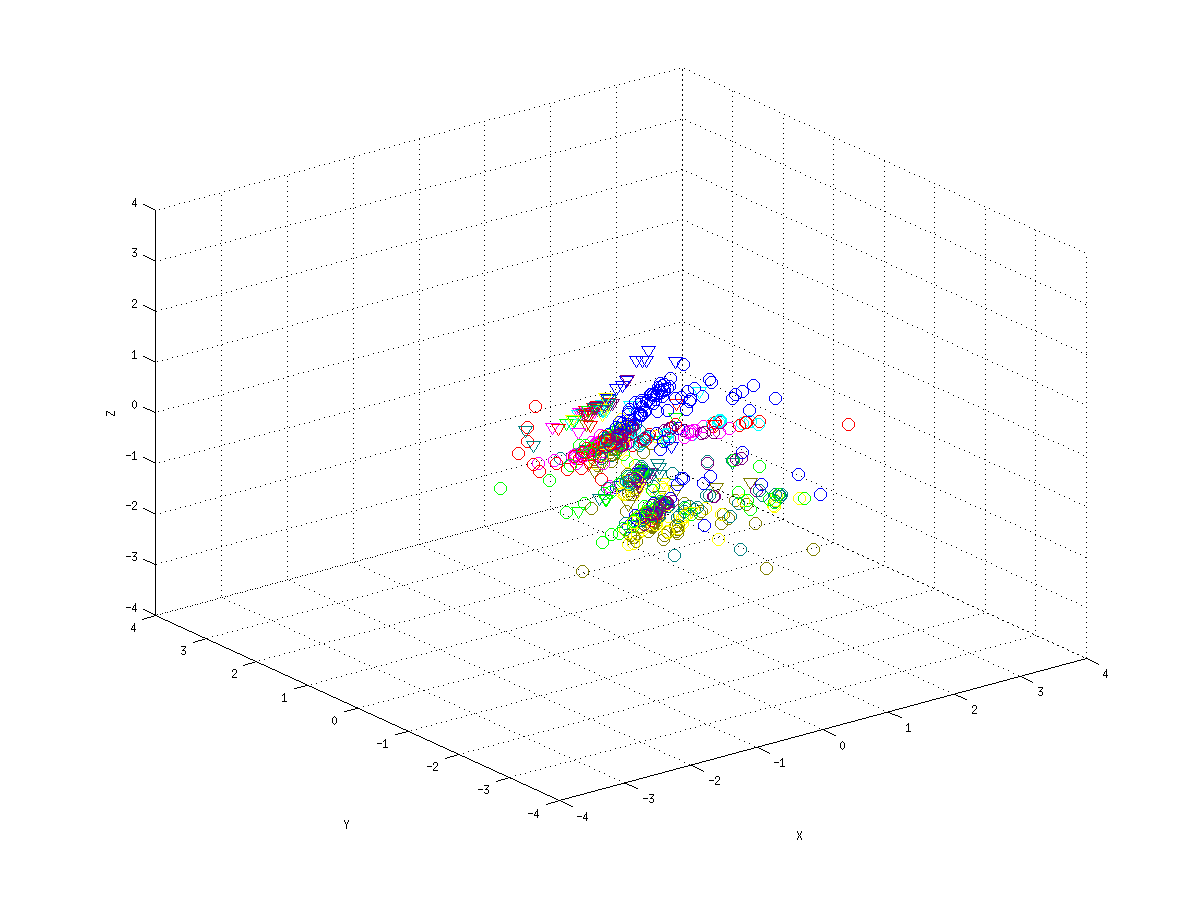
\includegraphics[width=\textwidth]{graficos/fold1_criterioParadao_reglaM_alpha0_rep1_0P.png}
                \caption{Vista en perspectiva.}
        \end{subfigure}%
        ~
        \begin{subfigure}[b]{0.49\textwidth}
                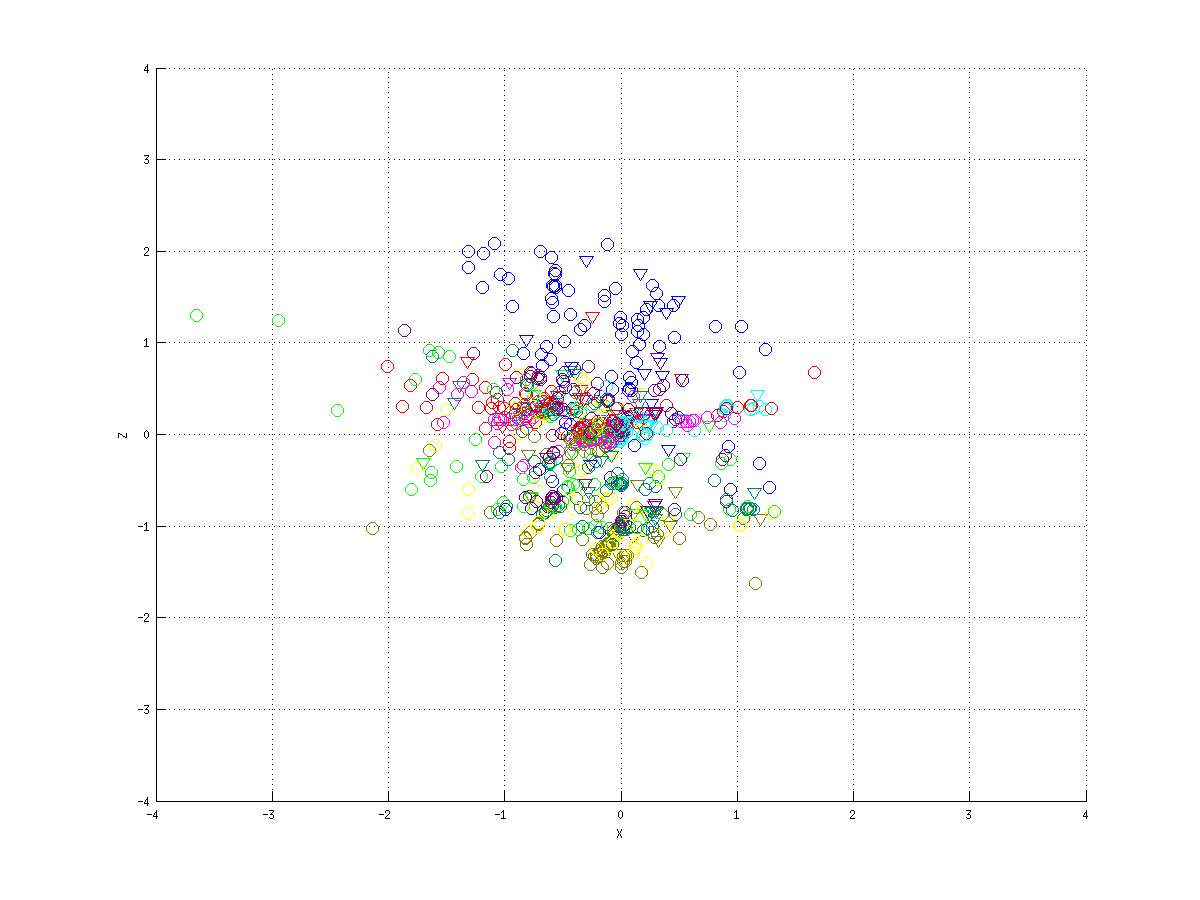
\includegraphics[width=\textwidth]{graficos/fold1_criterioParadao_reglaM_alpha0_rep1_1XZ.png}
                \caption{Plano X-Z.}
        \end{subfigure}
        
        \hspace*{-6.5cm}
        \begin{subfigure}[b]{0.49\textwidth}
                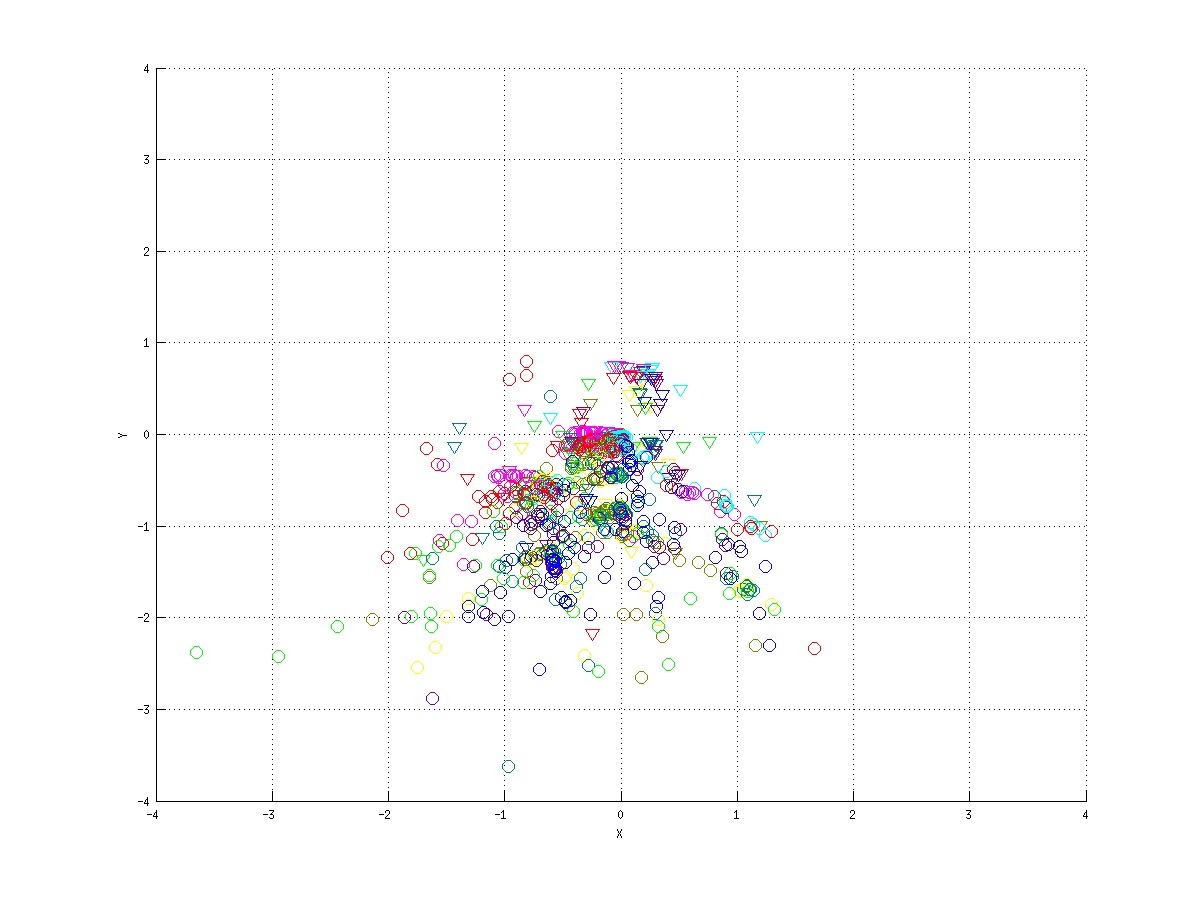
\includegraphics[width=\textwidth]{graficos/fold1_criterioParadao_reglaM_alpha0_rep1_2XY.png}
                \caption{Plano X-Y.}
        \end{subfigure}
        ~
        \begin{subfigure}[b]{0.49\textwidth}
                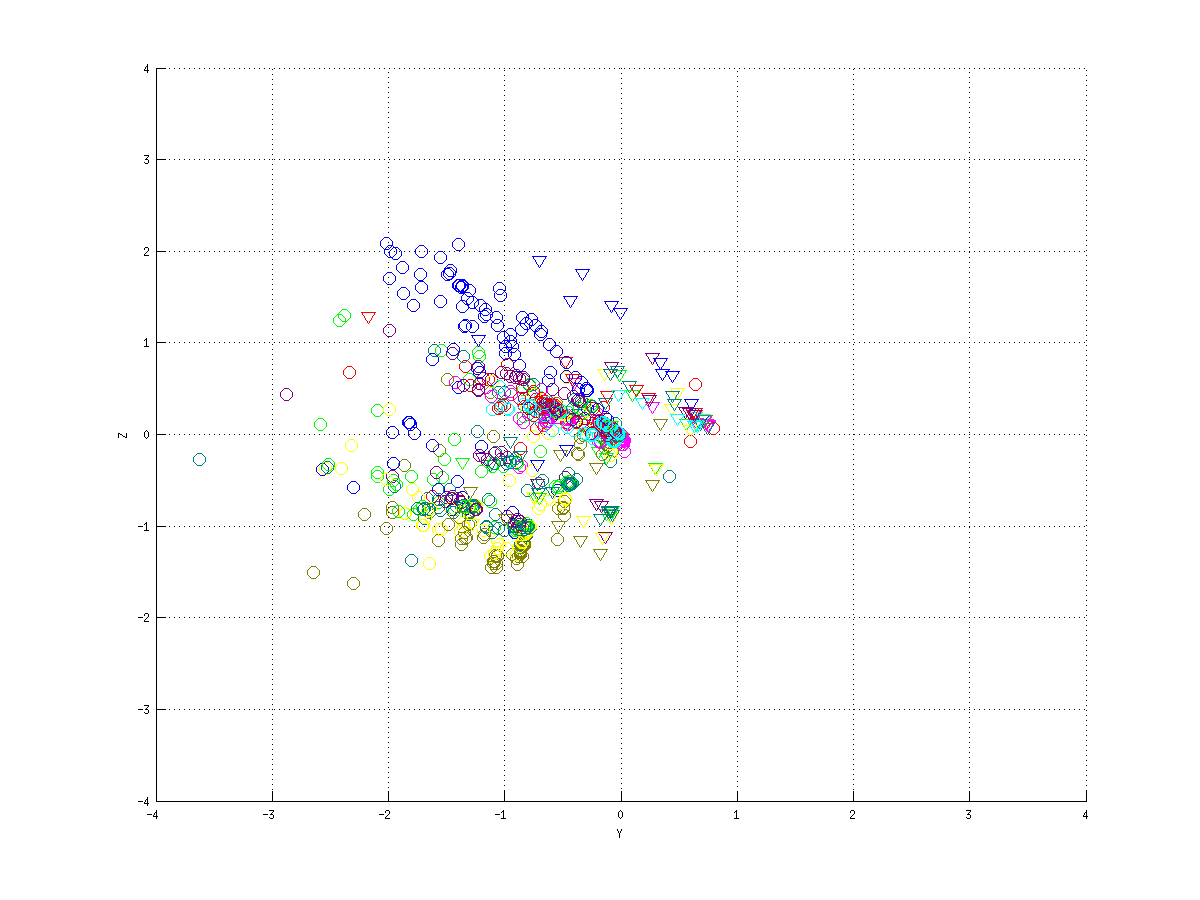
\includegraphics[width=\textwidth]{graficos/fold1_criterioParadao_reglaM_alpha0_rep1_3YZ.png}
                \caption{Plano Y-Z.}
        \end{subfigure}
	\restoregeometry
        \caption{Gráfico espacial para el Fold 1 usando ortogonalidad como criterio de parada y la regla de Oja con learning rate 0.001 en la repetición 1.}
        \label{fig:fold1_criterioParadao_reglaM_alpha0_rep1}
	\end{figure}
      
      
	\begin{figure}[H]
	\newgeometry{textwidth=21cm,textheight=21cm}
        \centering
        \hspace*{-6.5cm}
        \begin{subfigure}[b]{0.49\textwidth}
                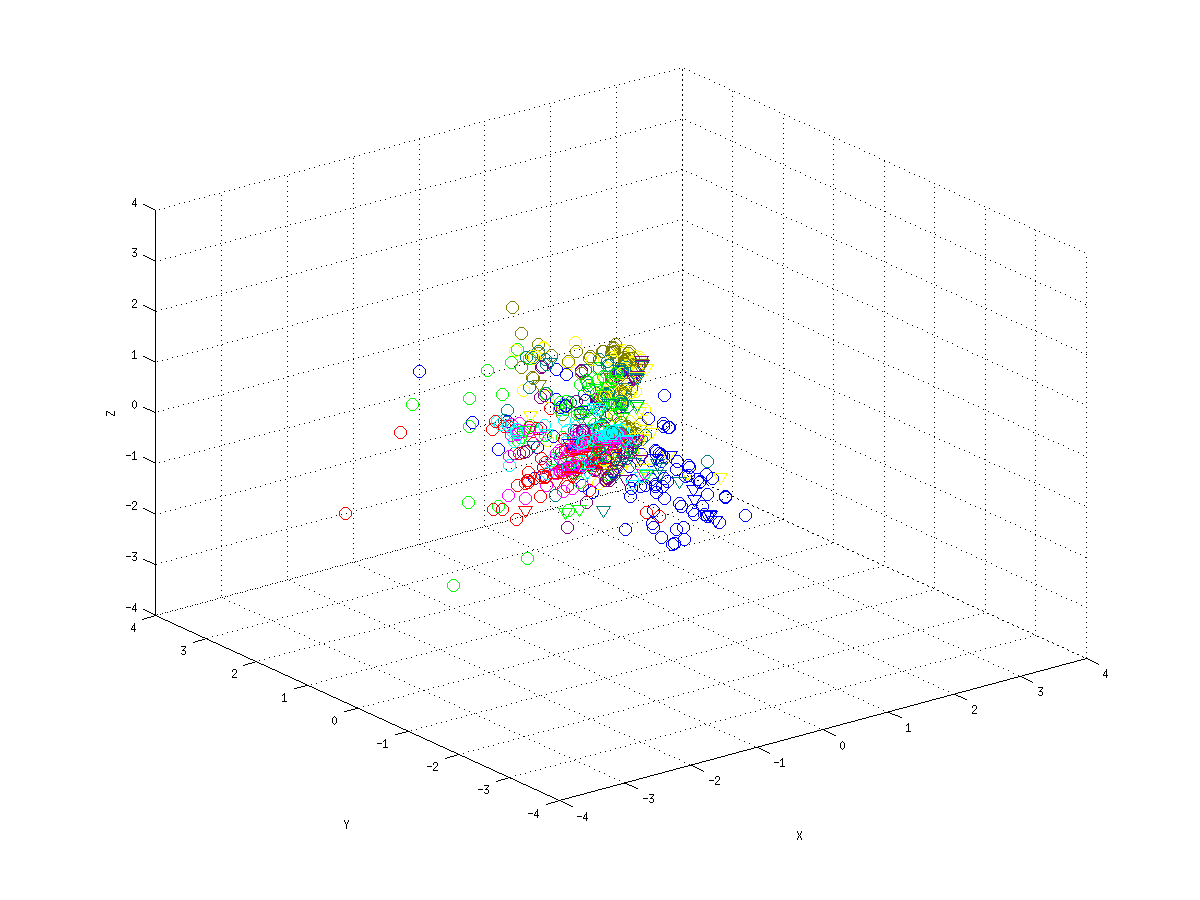
\includegraphics[width=\textwidth]{graficos/fold2_criterioParadao_reglaM_alpha0_rep1_0P.png}
                \caption{Vista en perspectiva.}
        \end{subfigure}%
        ~
        \begin{subfigure}[b]{0.49\textwidth}
                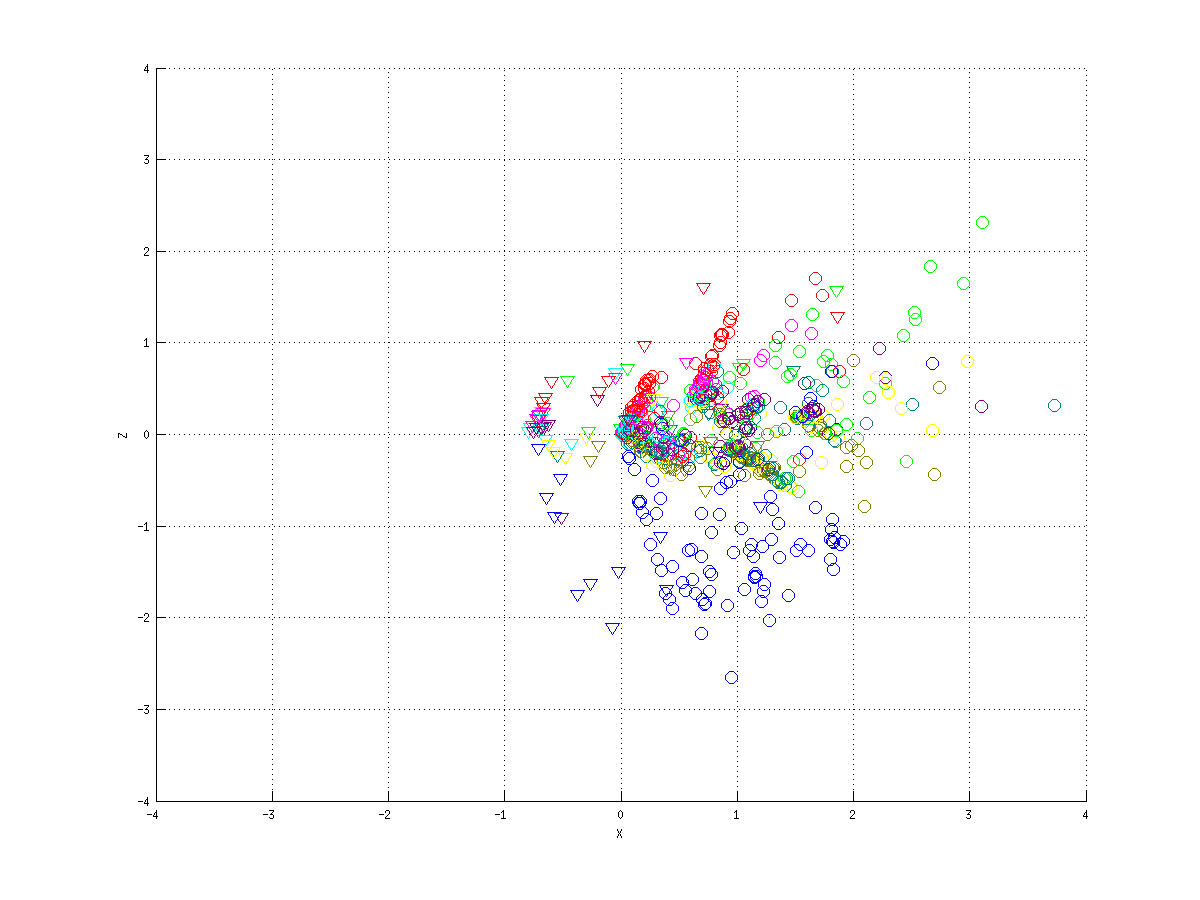
\includegraphics[width=\textwidth]{graficos/fold2_criterioParadao_reglaM_alpha0_rep1_1XZ.png}
                \caption{Plano X-Z.}
        \end{subfigure}
        
        \hspace*{-6.5cm}
        \begin{subfigure}[b]{0.49\textwidth}
                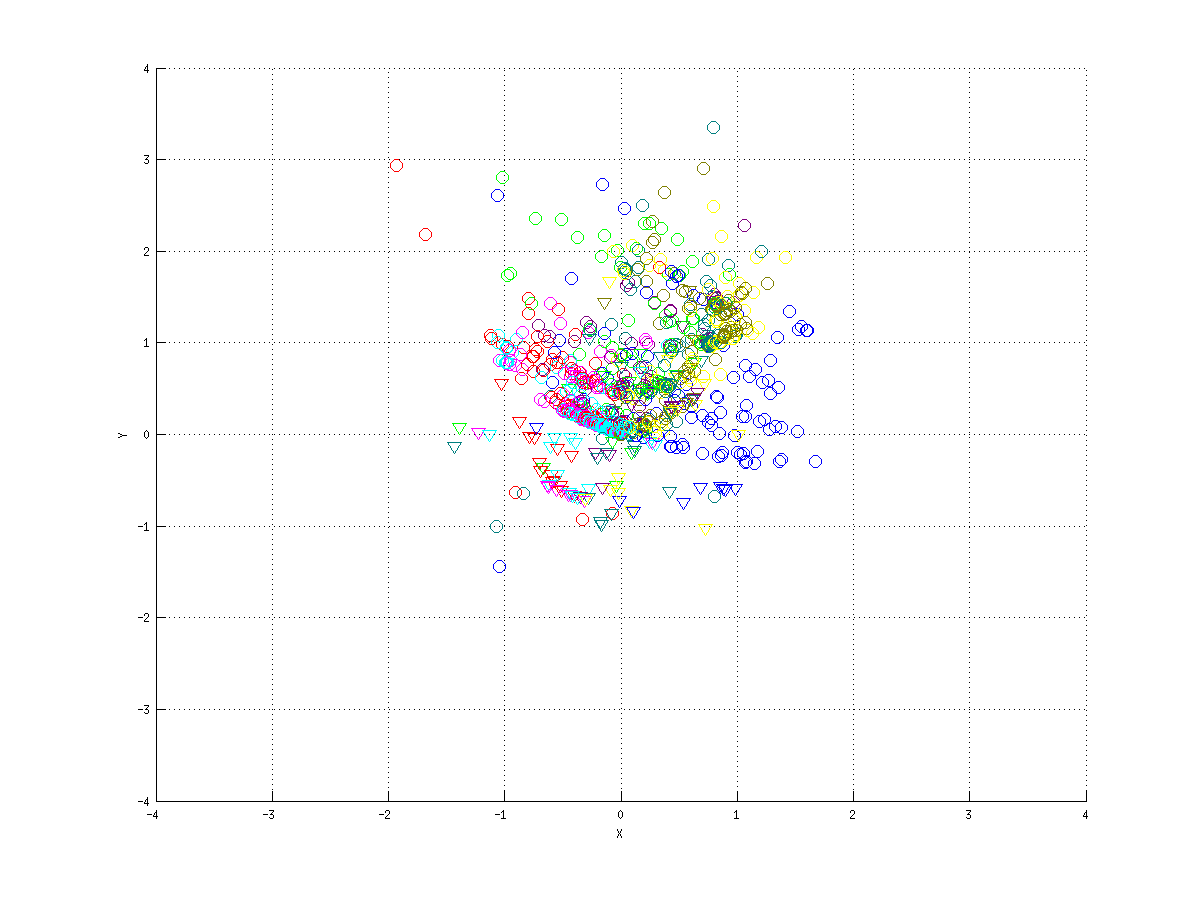
\includegraphics[width=\textwidth]{graficos/fold2_criterioParadao_reglaM_alpha0_rep1_2XY.png}
                \caption{Plano X-Y.}
        \end{subfigure}
        ~
        \begin{subfigure}[b]{0.49\textwidth}
                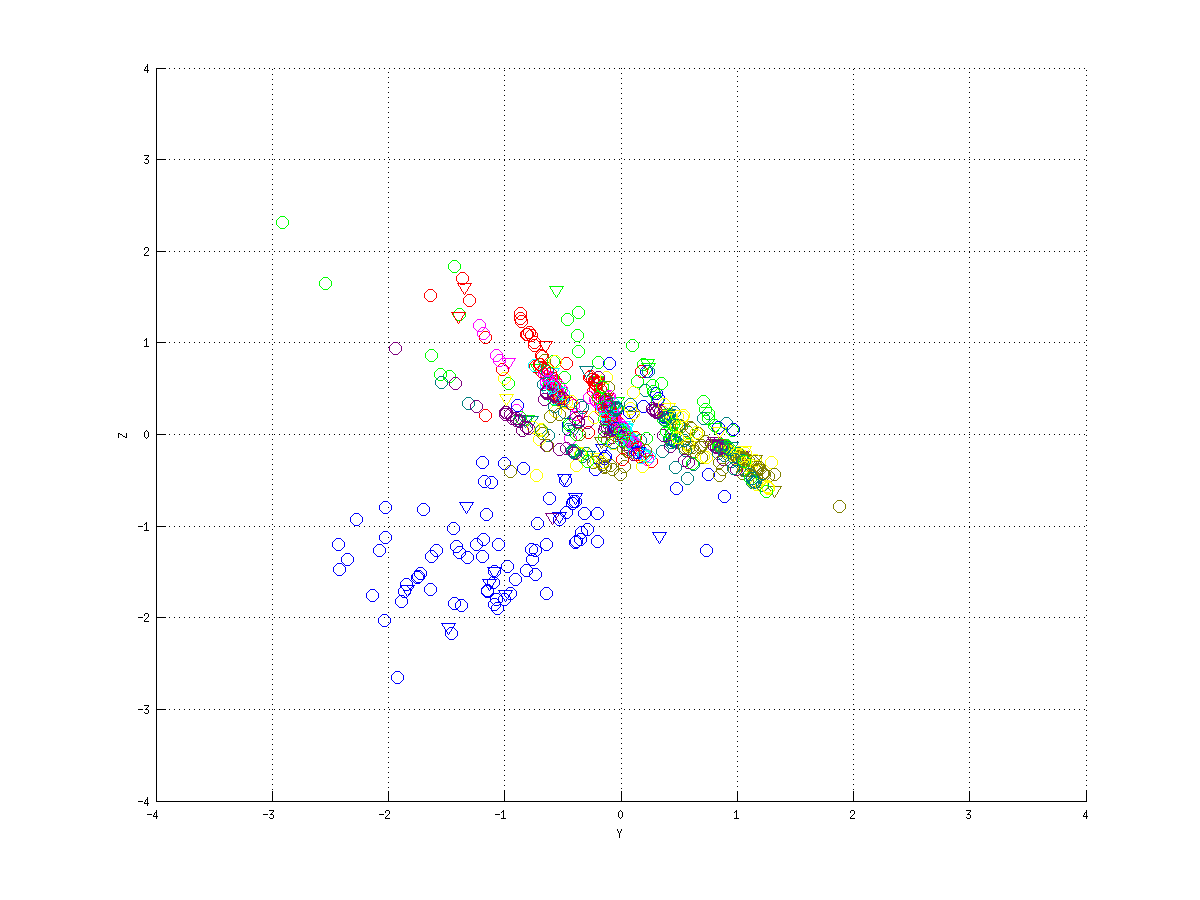
\includegraphics[width=\textwidth]{graficos/fold2_criterioParadao_reglaM_alpha0_rep1_3YZ.png}
                \caption{Plano Y-Z.}
        \end{subfigure}
	\restoregeometry
        \caption{Gráfico espacial para el Fold 2 usando ortogonalidad como criterio de parada y la regla de Oja con learning rate 0.001 en la repetición 1.}
        \label{fig:fold2_criterioParadao_reglaM_alpha0_rep1}
	\end{figure}      
      
      
      
      
      \myparagraph{Particularidades con regla de Sanger y criterio de ortogonalidad}
      
	Las Figuras \ref{fig:fold1_criterioParadao_reglas_alpha0_rep1} y \ref{fig:fold5_criterioParadao_reglas_alpha0_rep1} representan los dos tipos de comportamiento observados en general en todas las instancias experimentadas independientemente de si el criterio de corte fue que se alcanzó el máximo de épocas o que los vectores eran ortogonales. De manera similar a cuando se utiliza la regla de Oja, se puede ver aquí también dos -grupos de resultados similares. En la Figura \ref{fig:fold1_criterioParadao_reglas_alpha0_rep1} podemos ver que en general las instancias se encuentran agrupadas en una porción del espacio reducida y hay cúmulos de algunas clases como las representadas con los colores rojo, celeste, amarillo y verde. Otras clases como las expresadas con colores azul, violeta y rosa ocupan lugares espaciados y relativamente demarcados.
	
	En el caso de la Figura \ref{fig:fold5_criterioParadao_reglas_alpha0_rep1} las instancias se encuentran más separadas en general con cúmulos que agrupan varias clases por ejemplo donde se ubican las instancias rojas y celestes así como las amarillas y verdes. Respecto de las clases más separadas que ocupan espacios demarcados (azul y violeta), las mismas ocupan mayor espacio que en el otro caso.
      
      
	\begin{figure}[H]
	\newgeometry{textwidth=21cm,textheight=21cm}
        \centering
        \hspace*{-6.5cm}
        \begin{subfigure}[b]{0.49\textwidth}
                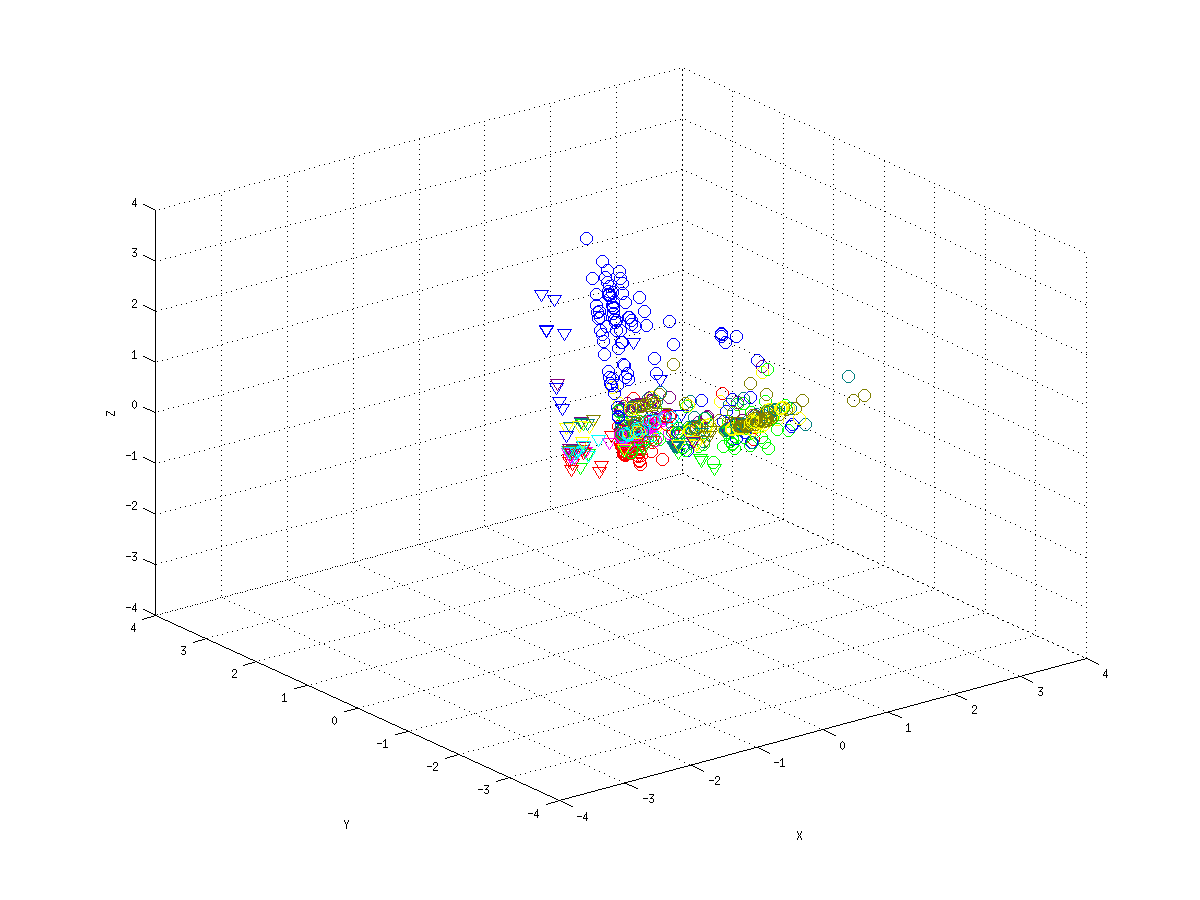
\includegraphics[width=\textwidth]{graficos/fold1_criterioParadao_reglas_alpha0_rep1_0P.png}
                \caption{Vista en perspectiva.}
        \end{subfigure}%
        ~
        \begin{subfigure}[b]{0.49\textwidth}
                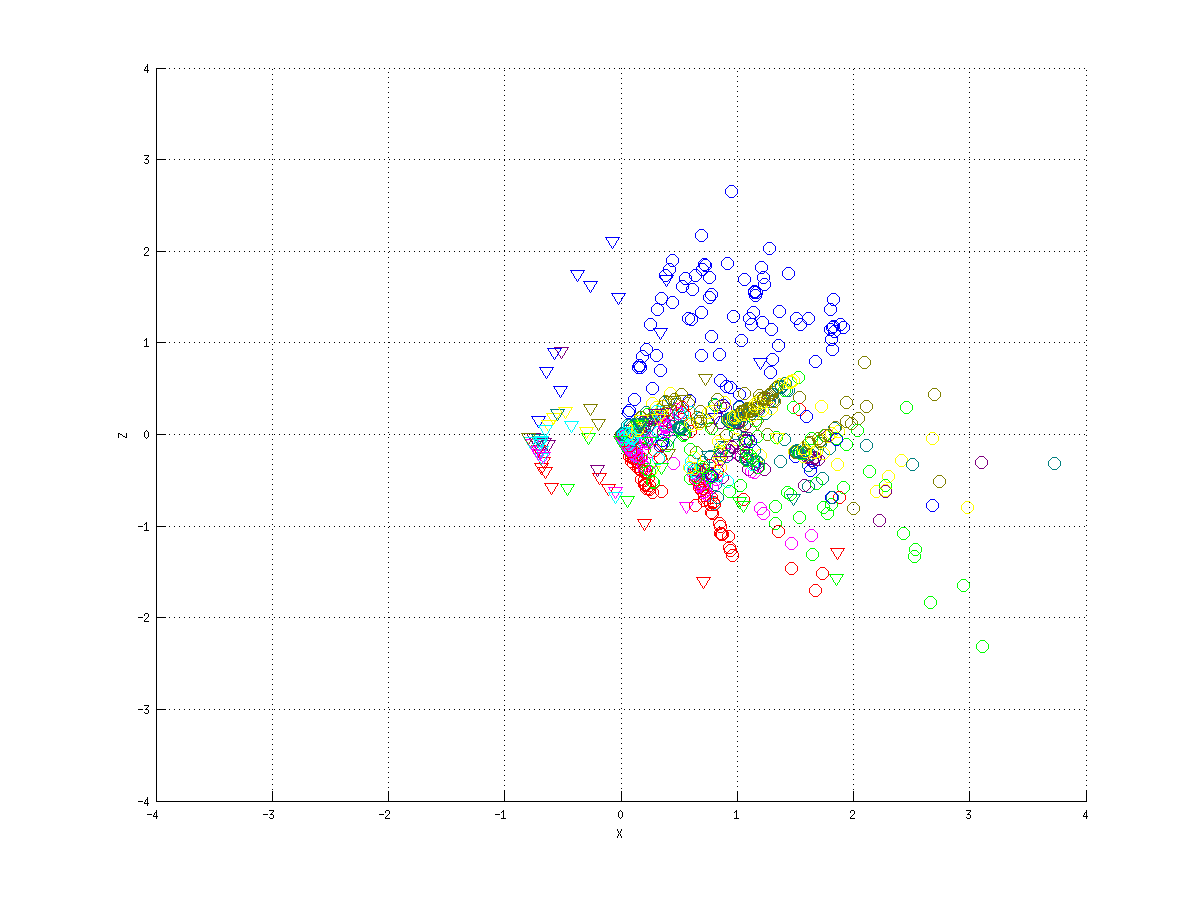
\includegraphics[width=\textwidth]{graficos/fold1_criterioParadao_reglas_alpha0_rep1_1XZ.png}
                \caption{Plano X-Z.}
        \end{subfigure}
        
        \hspace*{-6.5cm}
        \begin{subfigure}[b]{0.49\textwidth}
                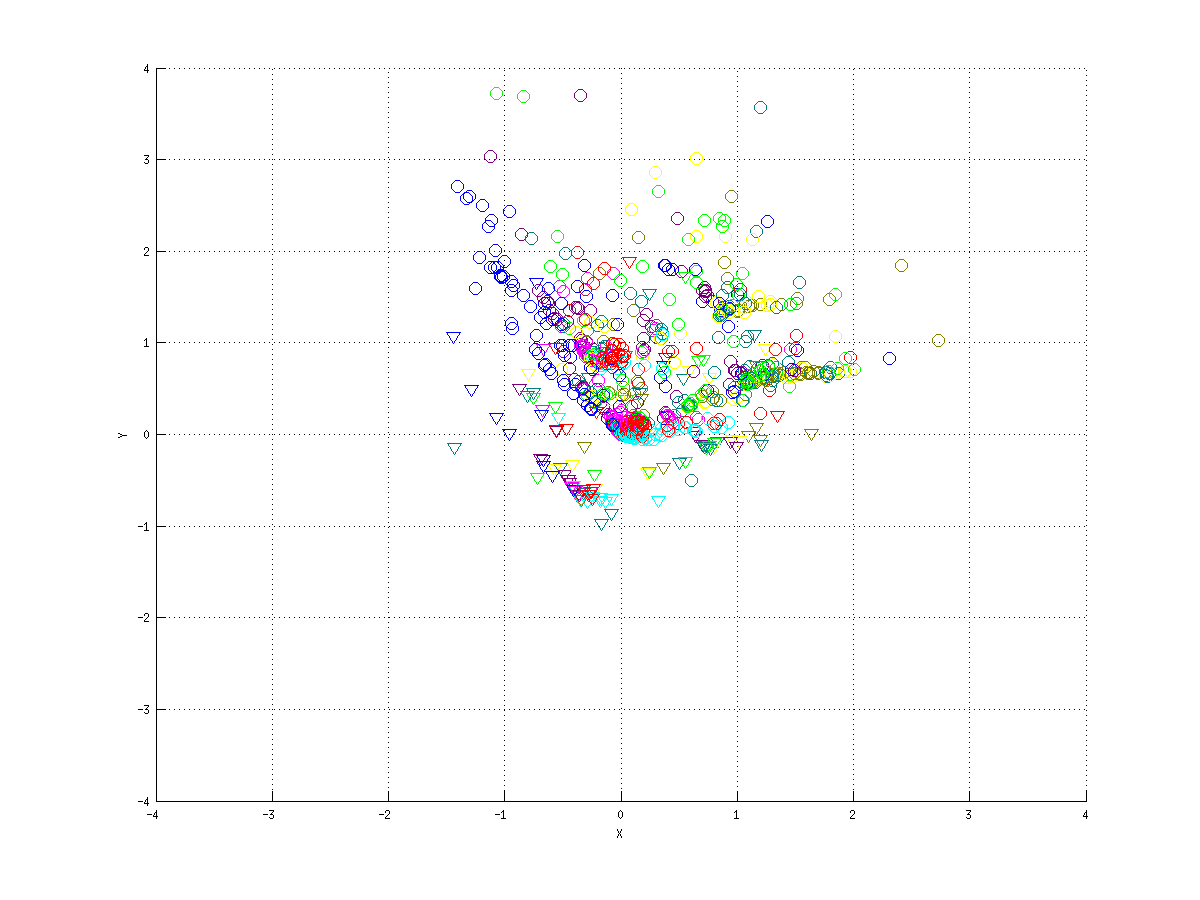
\includegraphics[width=\textwidth]{graficos/fold1_criterioParadao_reglas_alpha0_rep1_2XY.png}
                \caption{Plano X-Y.}
        \end{subfigure}
        ~
        \begin{subfigure}[b]{0.49\textwidth}
                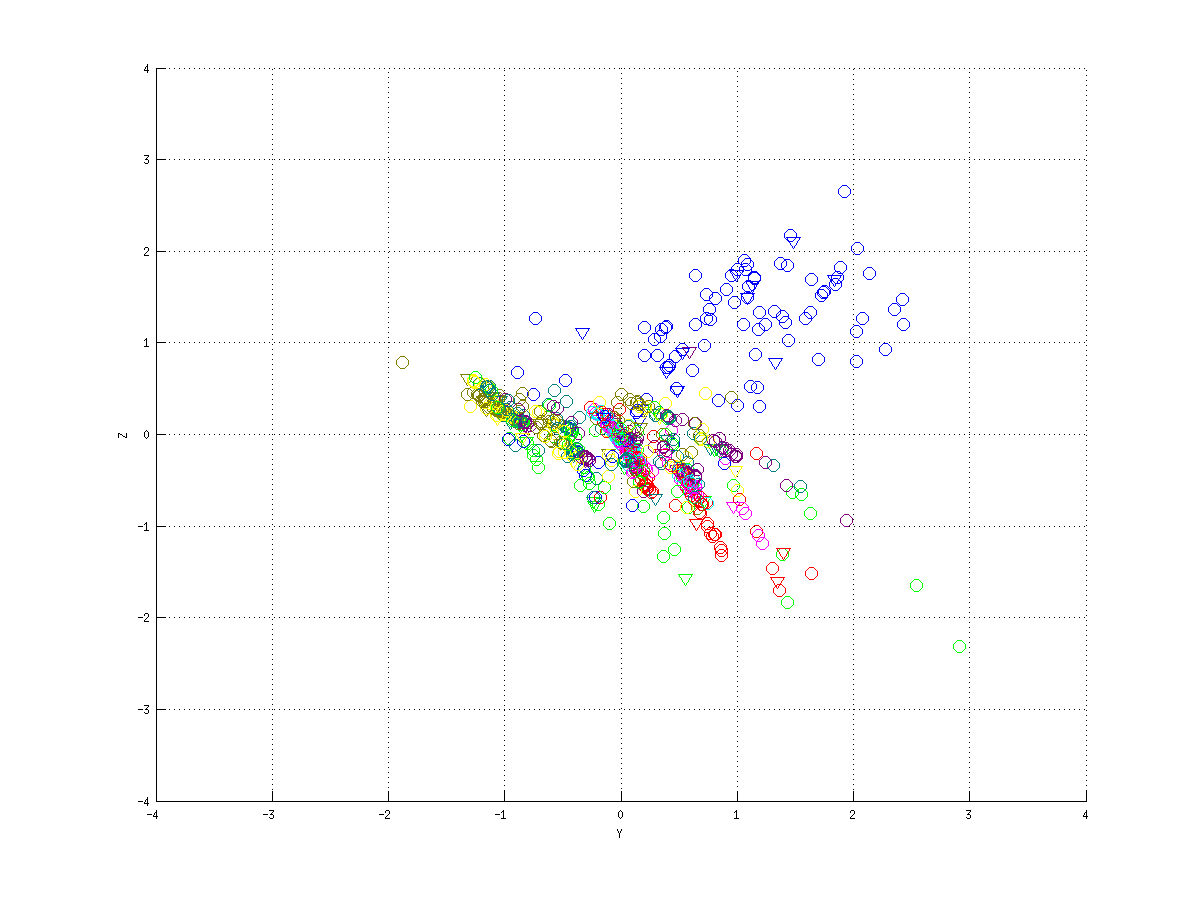
\includegraphics[width=\textwidth]{graficos/fold1_criterioParadao_reglas_alpha0_rep1_3YZ.png}
                \caption{Plano Y-Z.}
        \end{subfigure}
	\restoregeometry
        \caption{Gráfico espacial para el Fold 1 usando ortogonalidad como criterio de parada y la regla de Sanger con learning rate 0.001 en la repetición 1.}
        \label{fig:fold1_criterioParadao_reglas_alpha0_rep1}
	\end{figure}
      
	
	\begin{figure}[H]
	\newgeometry{textwidth=21cm,textheight=21cm}
        \centering
        \hspace*{-6.5cm}
        \begin{subfigure}[b]{0.49\textwidth}
                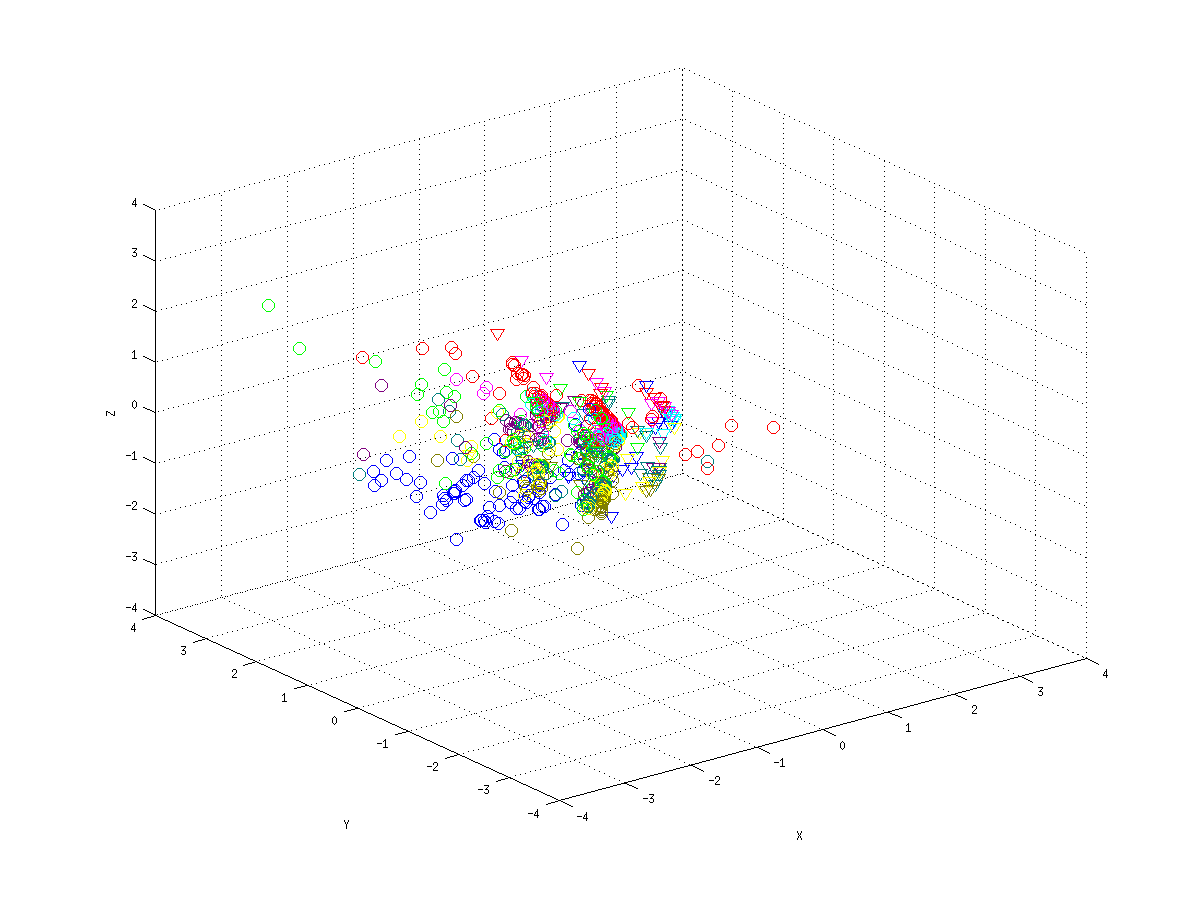
\includegraphics[width=\textwidth]{graficos/fold5_criterioParadao_reglas_alpha0_rep1_0P.png}
                \caption{Vista en perspectiva.}
        \end{subfigure}%
        ~
        \begin{subfigure}[b]{0.49\textwidth}
                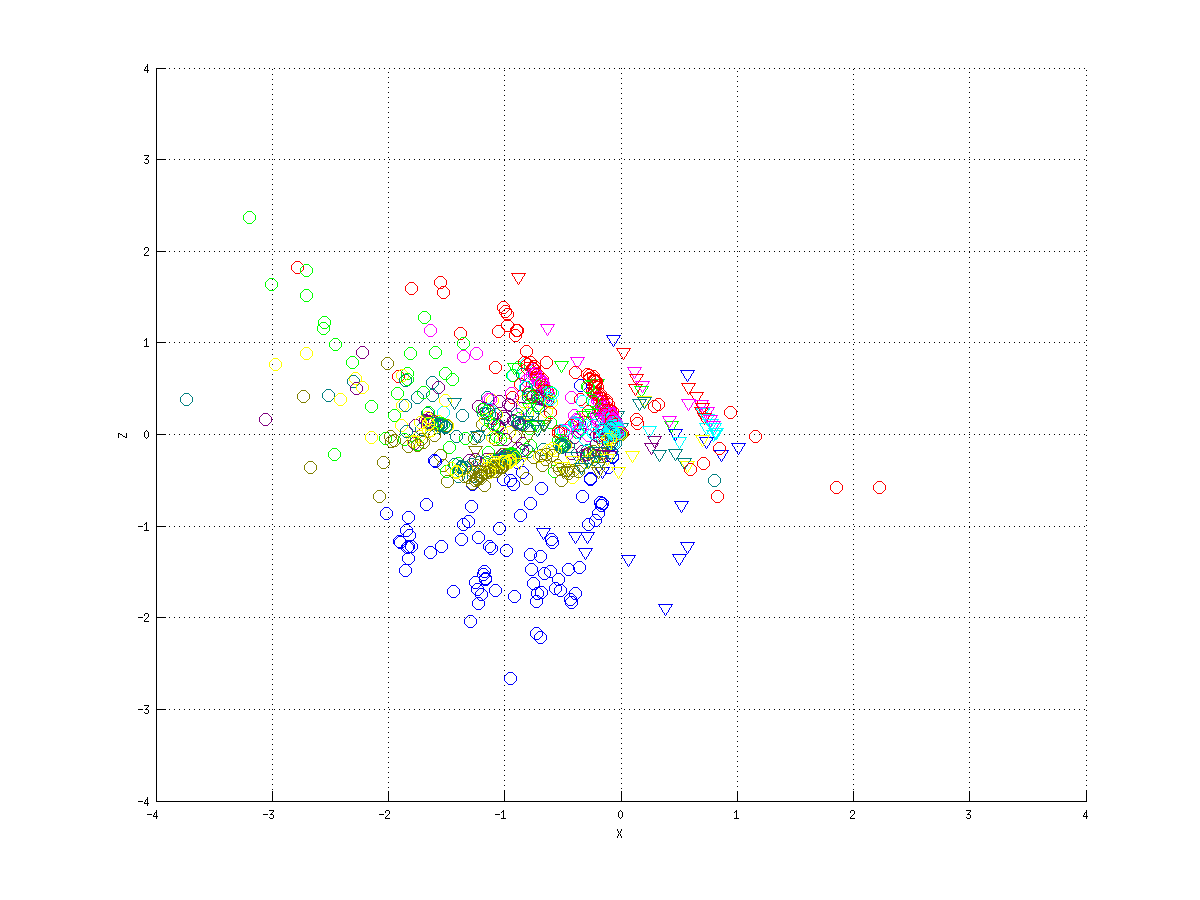
\includegraphics[width=\textwidth]{graficos/fold5_criterioParadao_reglas_alpha0_rep1_1XZ.png}
                \caption{Plano X-Z.}
        \end{subfigure}
        
        \hspace*{-6.5cm}
        \begin{subfigure}[b]{0.49\textwidth}
                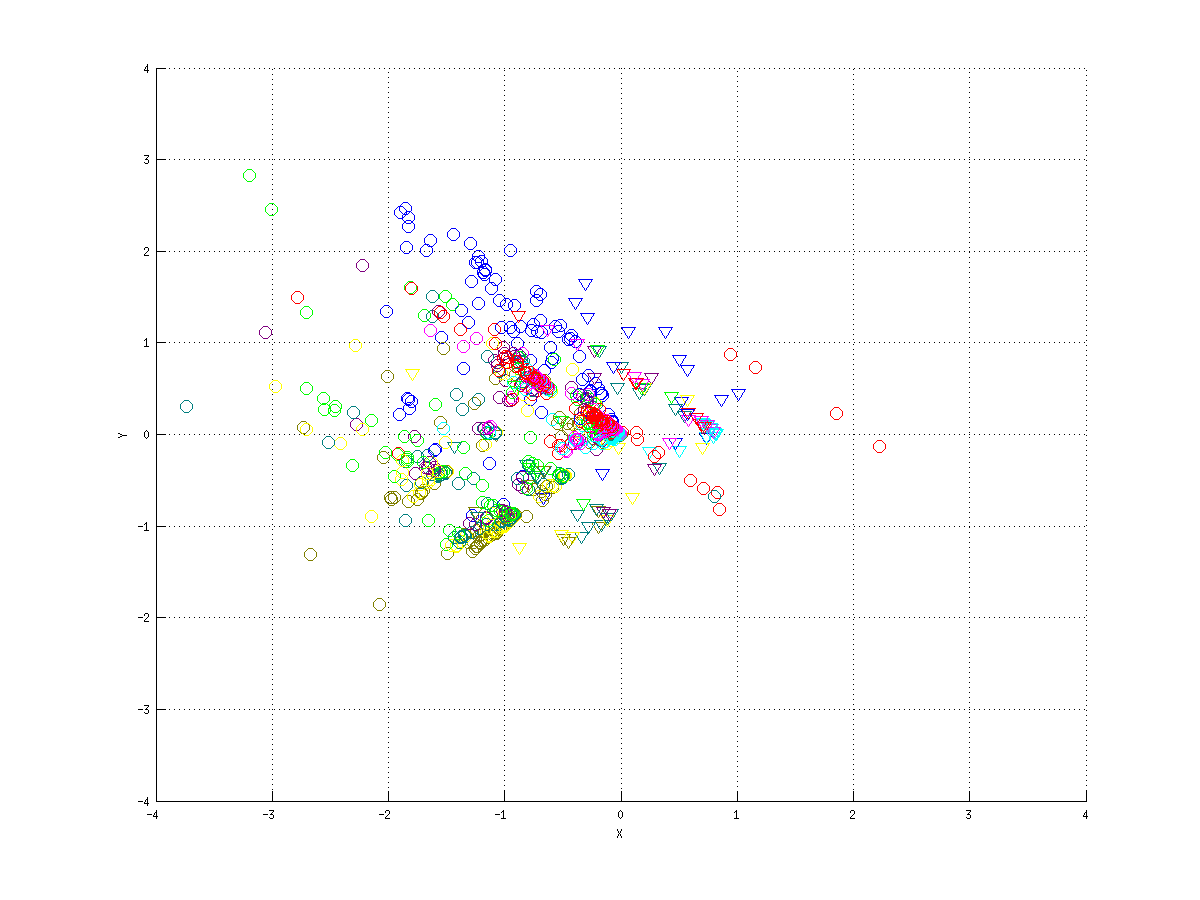
\includegraphics[width=\textwidth]{graficos/fold5_criterioParadao_reglas_alpha0_rep1_2XY.png}
                \caption{Plano X-Y.}
        \end{subfigure}
        ~
        \begin{subfigure}[b]{0.49\textwidth}
                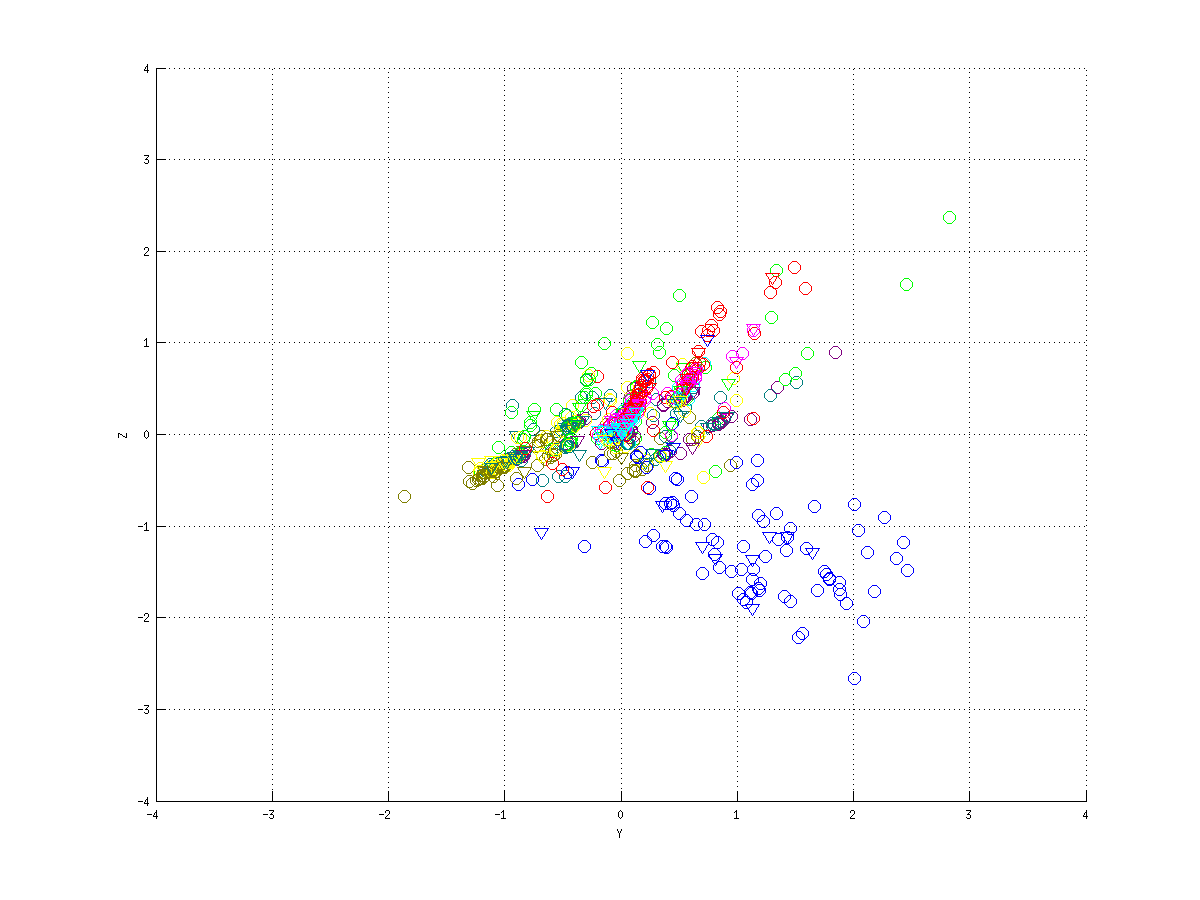
\includegraphics[width=\textwidth]{graficos/fold5_criterioParadao_reglas_alpha0_rep1_3YZ.png}
                \caption{Plano Y-Z.}
        \end{subfigure}
	\restoregeometry
        \caption{Gráfico espacial para el Fold 5 usando ortogonalidad como criterio de parada y la regla de Sanger con learning rate 0.001 en la repetición 1.}
        \label{fig:fold5_criterioParadao_reglas_alpha0_rep1}
	\end{figure}
      
      
      
      
      
      
      
      
      \myparagraph{Particularidades con regla de Oja y criterio de $\Delta W$}
      
	\begin{figure}[H]
	\newgeometry{textwidth=21cm,textheight=21cm}
        \centering
        \hspace*{-6.5cm}
        \begin{subfigure}[b]{0.49\textwidth}
                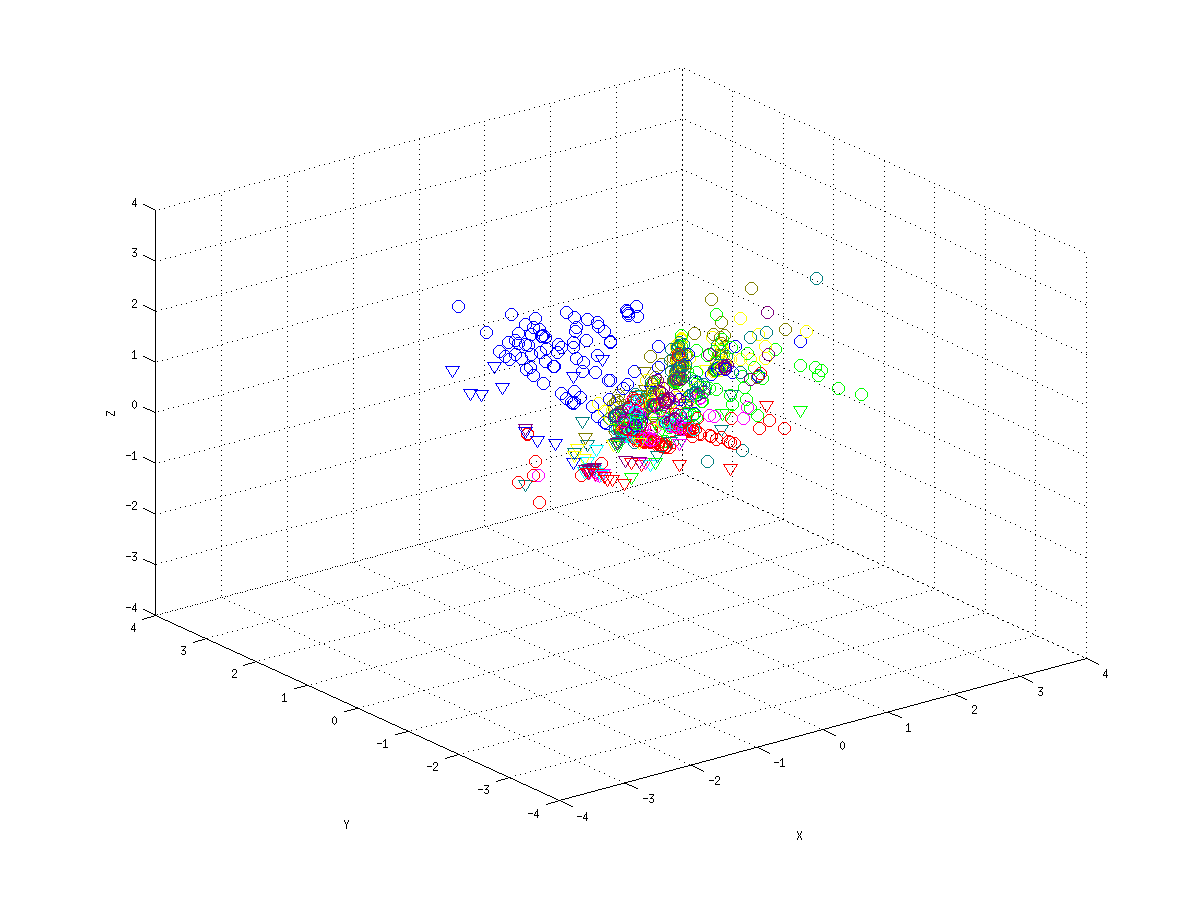
\includegraphics[width=\textwidth]{graficos/fold1_criterioParadap_reglaM_alpha0_rep1_0P.png}
                \caption{Vista en perspectiva.}
        \end{subfigure}%
        ~
        \begin{subfigure}[b]{0.49\textwidth}
                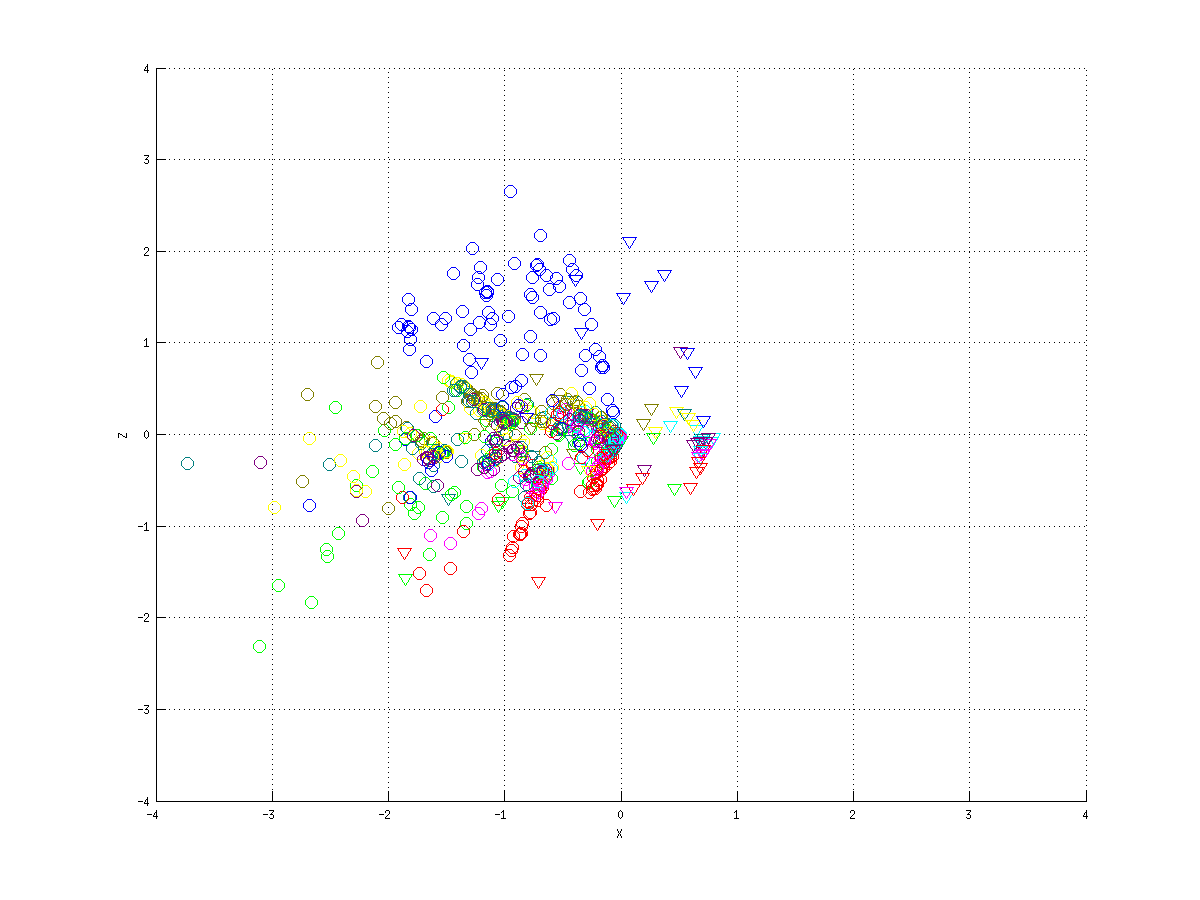
\includegraphics[width=\textwidth]{graficos/fold1_criterioParadap_reglaM_alpha0_rep1_1XZ.png}
                \caption{Plano X-Z.}
        \end{subfigure}
        
        \hspace*{-6.5cm}
        \begin{subfigure}[b]{0.49\textwidth}
                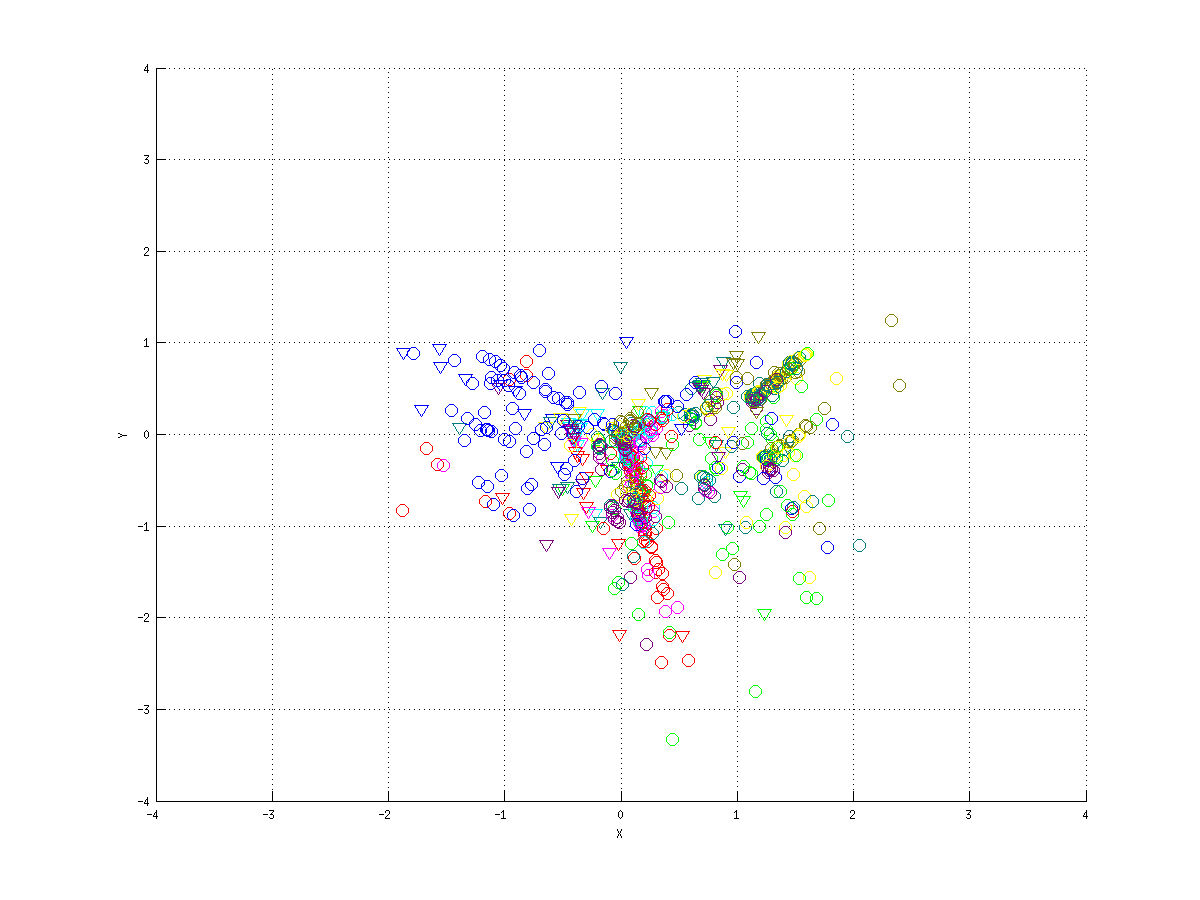
\includegraphics[width=\textwidth]{graficos/fold1_criterioParadap_reglaM_alpha0_rep1_2XY.png}
                \caption{Plano X-Y.}
        \end{subfigure}
        ~
        \begin{subfigure}[b]{0.49\textwidth}
                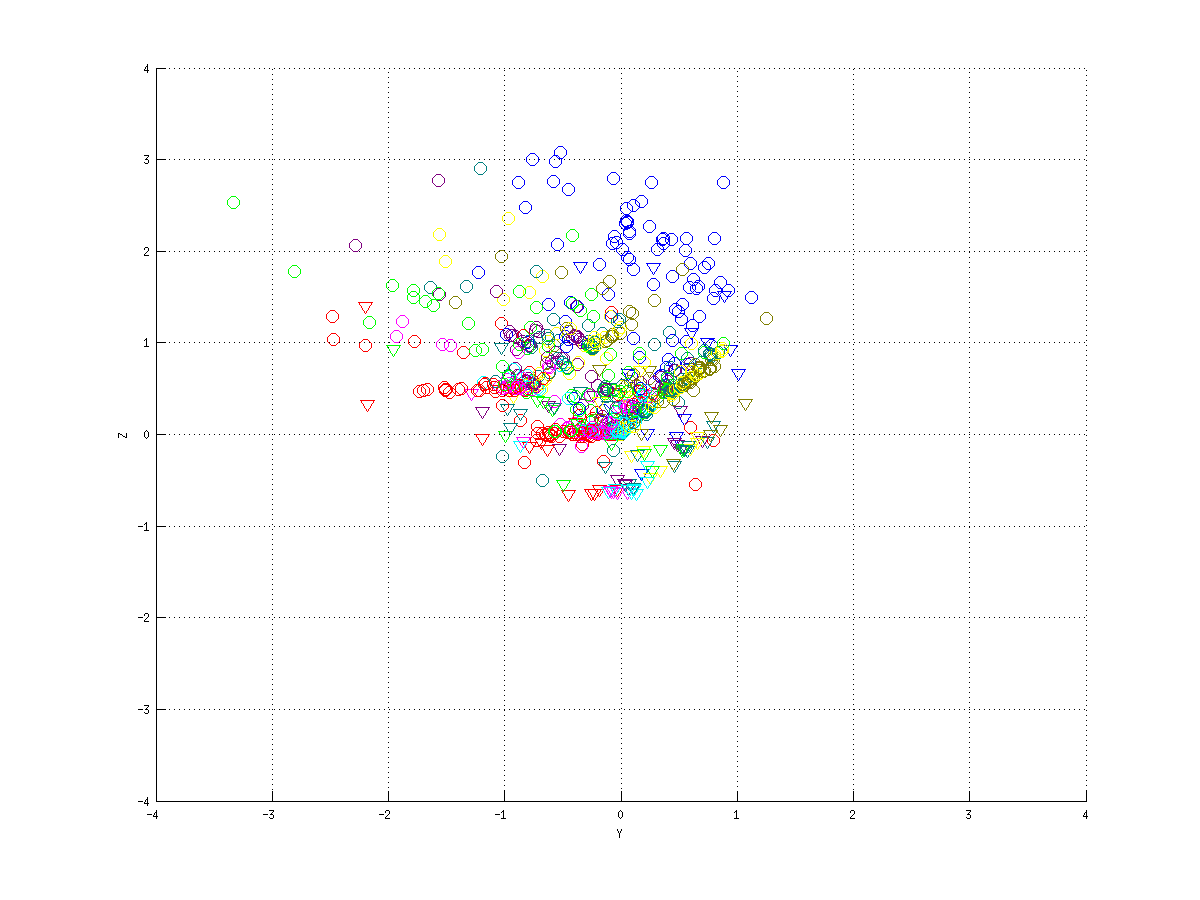
\includegraphics[width=\textwidth]{graficos/fold1_criterioParadap_reglaM_alpha0_rep1_3YZ.png}
                \caption{Plano Y-Z.}
        \end{subfigure}
	\restoregeometry
        \caption{Gráfico espacial para el Fold 1 usando $\Delta W$ como criterio de parada y la regla de Oja con learning rate 0.001 en la repetición 1.}
        \label{fig:fold1_criterioParadap_reglaM_alpha0_rep1}
	\end{figure}
      
      
      
      
      
      
      
      
      
      
      
      
      
      
      
      
      
      
      
      
      
      
      
	\begin{figure}[H]
	\newgeometry{textwidth=21cm,textheight=21cm}
        \centering
        \hspace*{-6.5cm}
        \begin{subfigure}[b]{0.49\textwidth}
                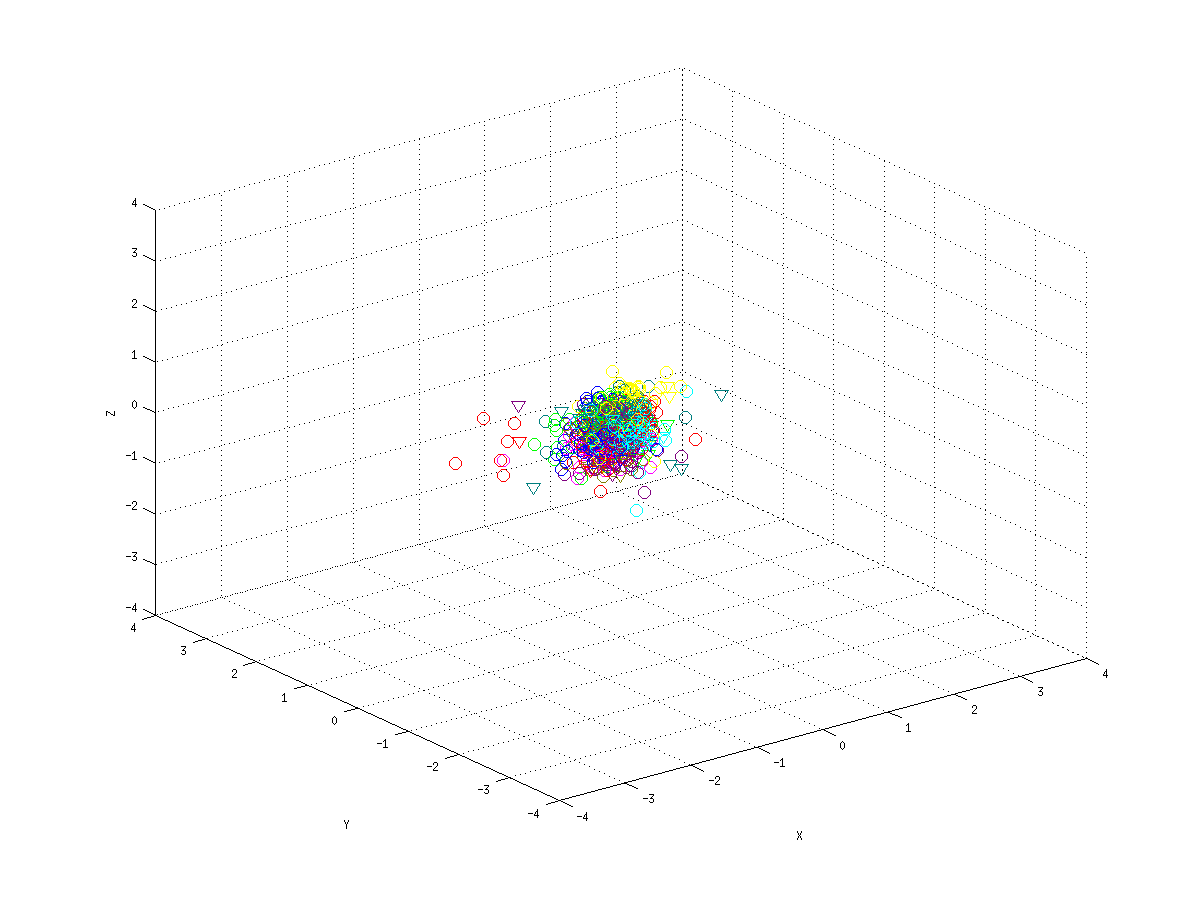
\includegraphics[width=\textwidth]{graficos/fold1_criterioParadap_reglas_alpha0_rep1_0P.png}
                \caption{Vista en perspectiva.}
        \end{subfigure}%
        ~
        \begin{subfigure}[b]{0.49\textwidth}
                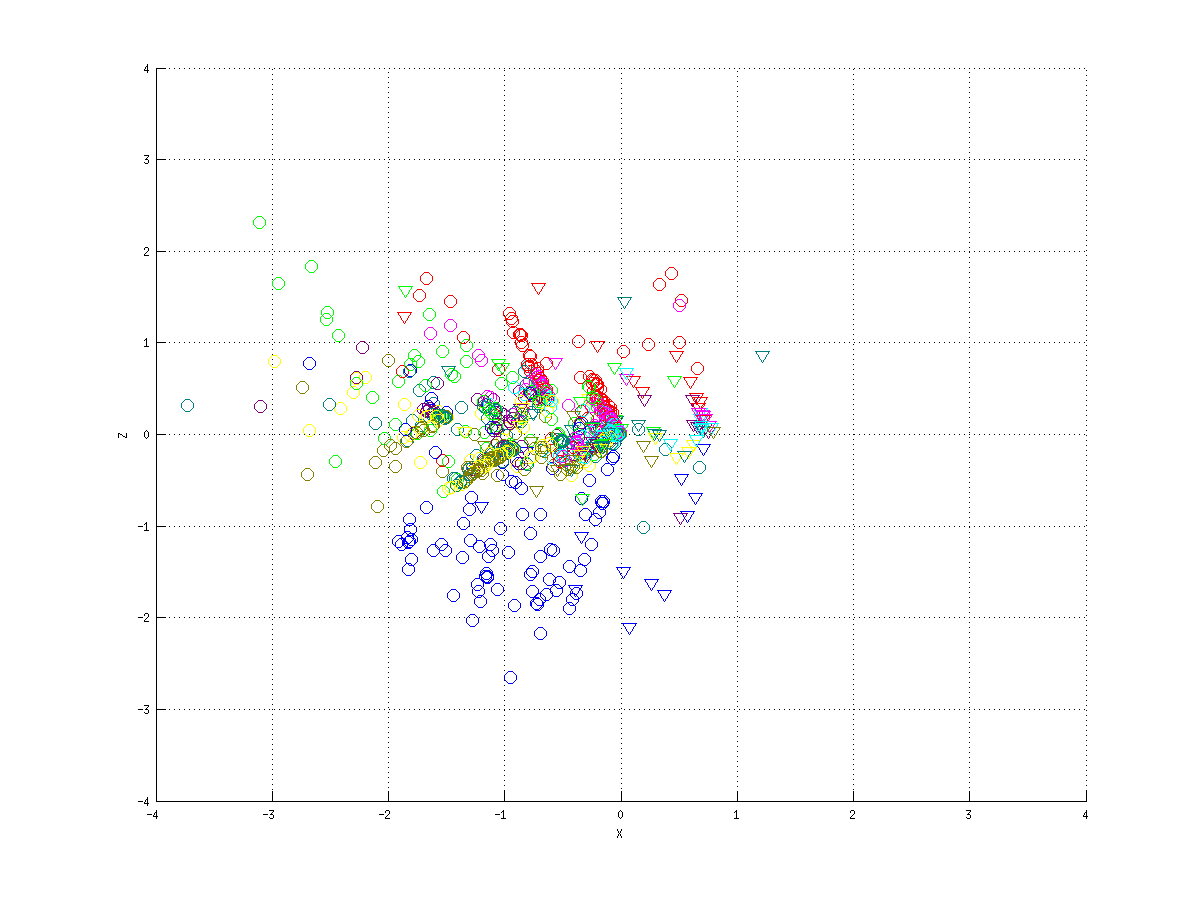
\includegraphics[width=\textwidth]{graficos/fold1_criterioParadap_reglas_alpha0_rep1_1XZ.png}
                \caption{Plano X-Z.}
        \end{subfigure}
        
        \hspace*{-6.5cm}
        \begin{subfigure}[b]{0.49\textwidth}
                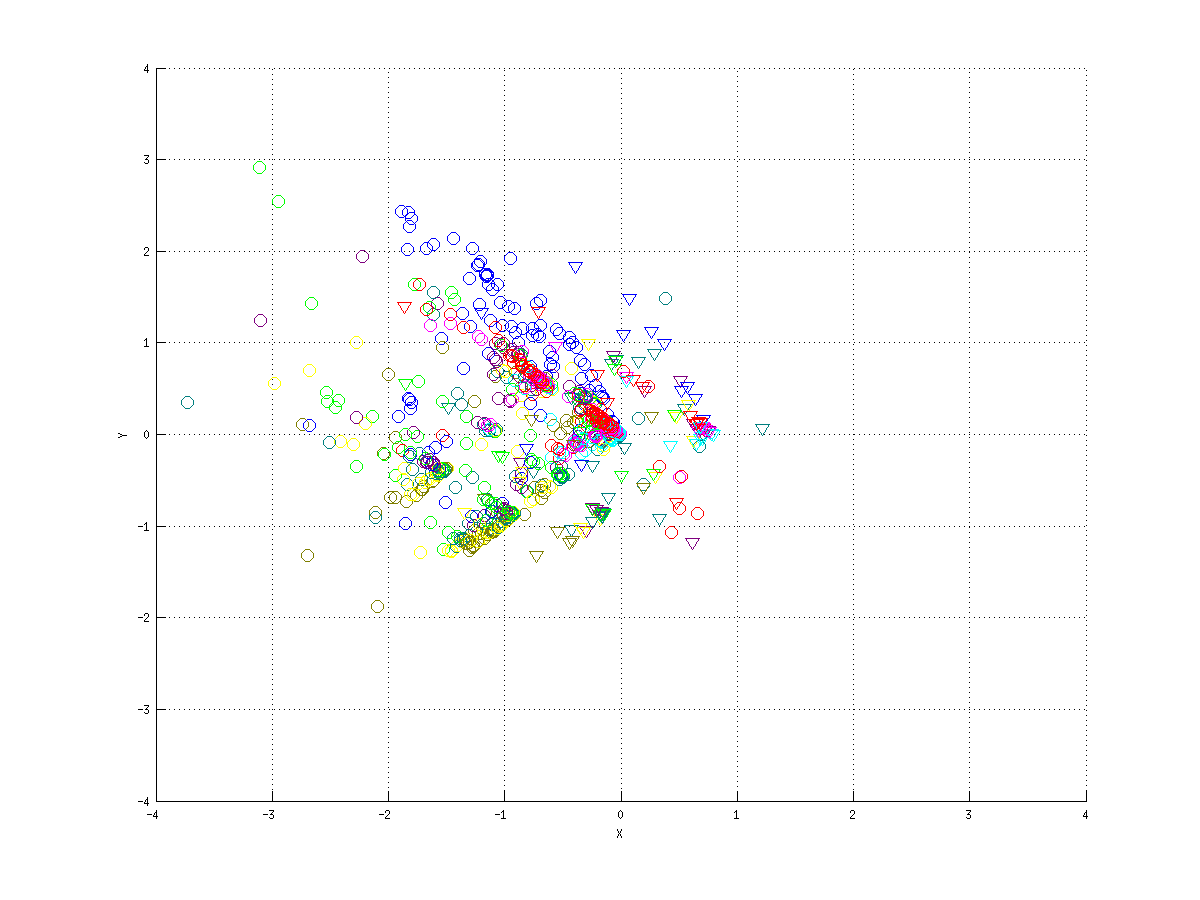
\includegraphics[width=\textwidth]{graficos/fold1_criterioParadap_reglas_alpha0_rep1_2XY.png}
                \caption{Plano X-Y.}
        \end{subfigure}
        ~
        \begin{subfigure}[b]{0.49\textwidth}
                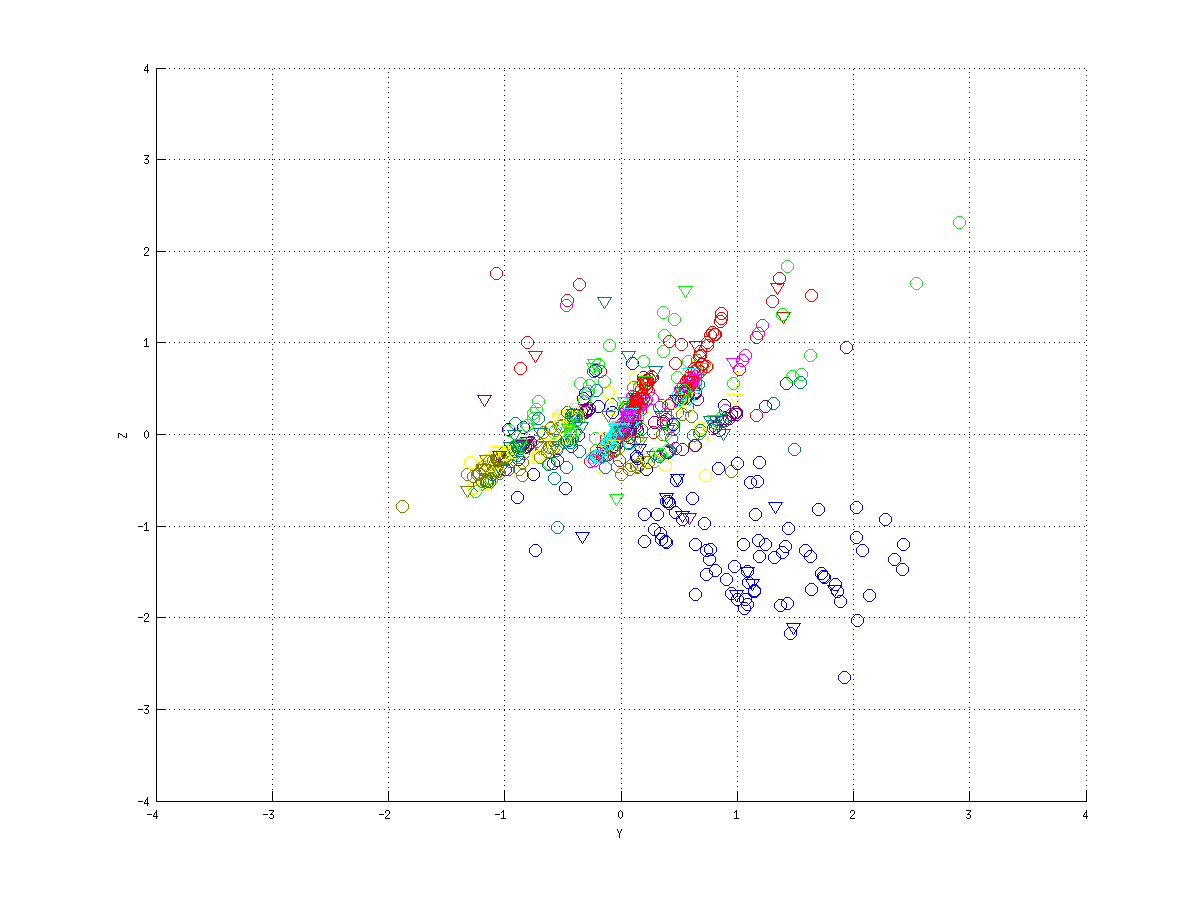
\includegraphics[width=\textwidth]{graficos/fold1_criterioParadap_reglas_alpha0_rep1_3YZ.png}
                \caption{Plano Y-Z.}
        \end{subfigure}
	\restoregeometry
        \caption{Gráfico espacial para el Fold 1 usando $\Delta W$ como criterio de parada y la regla de Sanger con learning rate 0.001 en la repetición 1.}
        \label{fig:fold1_criterioParadap_reglas_alpha0_rep1}
	\end{figure}
      
      
      
    \subsection{Mapeo de características}
    
      En este caso, el analisis de este modelo se vuelve algo particular. Para realizar el mismo, decidimos utilizar dos metricas: la primera con el objetivo de obtener alguna nocion de desempe\~no de la red, y la segunda para conocer que tan distanciados estaban los distintos grupos de activacion luego del entrenamiento.
      
      % TODO: (Para Rober) Explicar que son los dominantes en la seccion de desarrollo.
      
      \subsubsection{Distancia a dominantes}
      
      A la primera la llamaremos ``distancia a dominantes'' (DD) y representar\'a la distancia relativa media entre los dominantes del set de validaci\'on y el set de activaci\'on. Para generar su calculo, tomamos cada uno de los dominantes del mapa de validacion y buscamos el dominante mas cercano en el mapa de entrenamiento, en el mejor caso esta distancia es cero. 
      
      ~
      
      Obteniendo todas las distancias entre los distintos dominantes calcularemos su media y luego la normalizaremos diviendola por la distancia maxima que puede existir; esto es $||(M_1,M_2)||$, es decir la distancia entre las esquinas de la matriz de pesos.
      
      $$DD(DTr, DTe, W, M_1, M_2) = \frac{dM(mAct(DTr,W), mAct(DTe,W))}{||(M_1,M_2)||}$$
      
      Donde $DTr$ es el dataset de entrenamiento, $DTe$ es el dataset de validacion, $W$ es la matriz de pesos y $M_1, M_2$  son las dimensiones de la ultima. Se supone que $mAct$ calcula los mapas de dominantes para los datos otorgados y que $dM$ calcula la distancia media entre dichos dominantes.
      
      \subsubsection{Factor de cruce}
      
      La segunda ser\'a denominada como ``factor de cruce'' (FC) y nos dara una nocion de cuantas neuronas se activan mas de una clase. Esto nos sirve para observar de que forma la red neuronal esta respondiendo a distintos impulsos. Inferimos que es deseable que este factor sea bajo, ya que lo ideal seria que las distintas clases activen grupos de neuronas disjuntas.
      
      ~
      
      Para calcular este factor, nos armaremos un mapa de la red neuronal en donde tendremos registradas las cantidades de veces que se activo una neurona en las 9 clases distintas. En un escenario ideal, ningun numero deberia ser mayor a 1, ya que indicaria que una neurona se activo para mas de una clase.
      
      ~
      
      Una vez calculado este mapa sumaremos todos los valores de la matriz, le restaremos la cantidad de neuronas que no eran cero dentro del mapa (por lo que en el caso ideal el factor nos daria cero) y lo dividiremos por esa misma cantidad.
      
      $$FD(D, W) = \frac{sumActCruz(D, W) - noSonCero(D, W)}{noSonCero(D, W)}$$
      
      Donde $D$ representa los datos a utilizar y $W$ la matriz de pesos de la red neuronal ya entrenada. Se supone que $sumActCruz$ internamente calcula las activaciones, al igual que $noSonCero$ calcula la cantidad de neuronas que se activaron.
      
      ~
      \subsubsection{Analisis de resultados}
      Analizar los resultados de las metricas decidimos generar 9 folds distintos para luego promediar los resultados de los mismos. Cada fold tendra un set de entrenamiento y uno de validación generados al azar.
    
      %Para realizar el modelo se consideraron distintos tamaños de mapa así como también la opción de tener parámetros de aprendizaje autoajustables. El objetivo es tener un criterio comparativo para determinar qué tamaño es suficiente en relación a la cantidad de parámetros de las instancias.
      
      %Por otro lado, una vez generados los mapas con el conjunto de entrenamiento, el objetivo es catalogar las instancias del conjunto de validación usando los pesos y el mapa entrenados. 
      

\end{document}
\newpage

\section{Conclusiones}
\documentclass[informe.tex]{subfiles}
\begin{document}
  
  \section{Conclusiones}

\end{document}
\newpage

\section{Opciones de uso}
\documentclass[informe.tex]{subfiles}
\begin{document}
  
  \section{Opciones de uso}
  
    El código principal para el funcionamiento de la red se encuentra en MyMultiPerceptron.m como fue explicado en el desarrollo del trabajo. Sin embargo, existen dos archivos que buscan facilitar la obtenci\'on de resultados de entrenamiento y validaci\'on de la red. A continuaci\'on detallamos las funciones en esos dos archivos.
    
    \subsection{Training}
    
    Realiza el entrenamiento de una red dado un conjunto de parámetros elegidos y genera un gráfico del error según la época.
    
    ~
    
    \verb|function [ep_errors, final_error] = training(training_filename, hlayers, mode, | \\
    \verb|           output_filename, epochs, max_error, gamma, graph_filename, momentum)|
    
    \begin{itemize}
     \item \verb|training_filename| es el nombre del archivo a utilizar para entrenar. Por ejemplo, uno de los generados en las particiones.
     
     \item \verb|hlayers| es el vector con las capas ocultas que se quiere en la red. Por ejemplo, \verb|[2]| si se quieren dos neuronas en la capa oculta. Notemos que las cantidades de neuronas en las capas ocultas son independientes de las cantidades de entradas y salidas, las cuales son inferidas directamente de las dimensiones de los datasets.
    
     \item \verb|mode| es alguna variante para indicar la elección entre binaria o bipolar o regresión. Sus opciones son: ``bipolar'', ``binary'', ``bipolar-regresion'', ``binary-regresion''. Los \'ultimos dos difieren en los primeros utilizando una funcion lineal en la ultima capa. Este modo es necesario para el ejercicio 2.
    
     \item \verb|output_filename| es el nombre del archivo donde se guardarán los parámetros de la red entrenada.
    
     \item \verb|epochs| es el número máximo de épocas que se admite en el entrenamiento.
    
     \item \verb|max_error| es el error m\'aximo que se admite en el entrenamiento. Si el error de la red esta por debajo de este valor, el entrenamiento se detiene.
    
     \item \verb|gamma| es el learning rate.
    
     \item \verb|graph_filename| es el nombre del archivo donde se guardará el gráfico de error en función de las épocas.
     
     \item \verb|momentum| es el valor del momentum. Este par\'ametro es opcional, de no ingresarse el valor se define en cero.

     \item \verb|ep_errors| es el vector que guarda para cada época el error en esa etapa para el conjunto de entrenamiento mientras que \verb|final_error| es el \'ultimo valor del vector anterior.
    
    \end{itemize}
    
    \subsection{Testing}
    
    Lee los datos sobre una red entrenada y calcula el error sobre un conjunto de datos de testing.
    
    ~
    
    \verb|function error = testing(testing_filename, input_filename, gamma)|
    
    \begin{itemize}
      \item \verb|testing_filename| es el nombre del archivo sobre el cual se testeará la red.
      
      \item \verb|input_filename| es el archivo con los parámetros de la red entrenada.
      
      \item \verb|gamma| se utiliza para crear la instancia de la red.
      
      \item \verb|error| es el cálculo del error sobre el conjunto de validación.
    \end{itemize}
    
\end{document}


\end{document}
